

\documentclass[12pt]{report}

\usepackage{graphicx}
\title{Lab Report and Assignment}
\author{Samvram Sahu, SC15B132}

\begin{document}
\begin{titlepage}
	\centering
	
\includegraphics[width=0.5\linewidth]{skylark.png}\par\vspace{1cm}
	{\scshape\LARGE Automation of Auto-Pilot data transfer \par}
	\vspace{1cm}
	{\scshape\Large With the advent of Intel Edison  \par}
	\vspace{1.5cm}
	{\huge\bfseries A study report on application prospective \par}
	\vspace{1cm}
	{\Large\itshape Samvram Sahu\par}
	Drone Electronics Intern\\
	{\large \today\par}
\end{titlepage}

\tableofcontents

\chapter{The Problem Statement}
The use of PixHawk 1 in Skylark Drones is basically due to its unmatched versatility and efficiency. However the production of the same has come to an unforeseen halt with the advent of the PixHawk 2.1 and with the new board comes a whole new package of possibilities. With this being the context I am to:-
\begin{itemize}
 \item{Explore the possibilities along with Intel Edison as a parallel processor.}
 \item{Figure out a way to transmit the dataflash log to Ground Station(GS)}
 \item{Transfer the pictures to the Ground Station from Camera}
 \item{Explore Emlid Reach RTK module in the context of data transfer}
\end{itemize}
\vspace{6cm}

\chapter{Present Network}
\section{The connections}
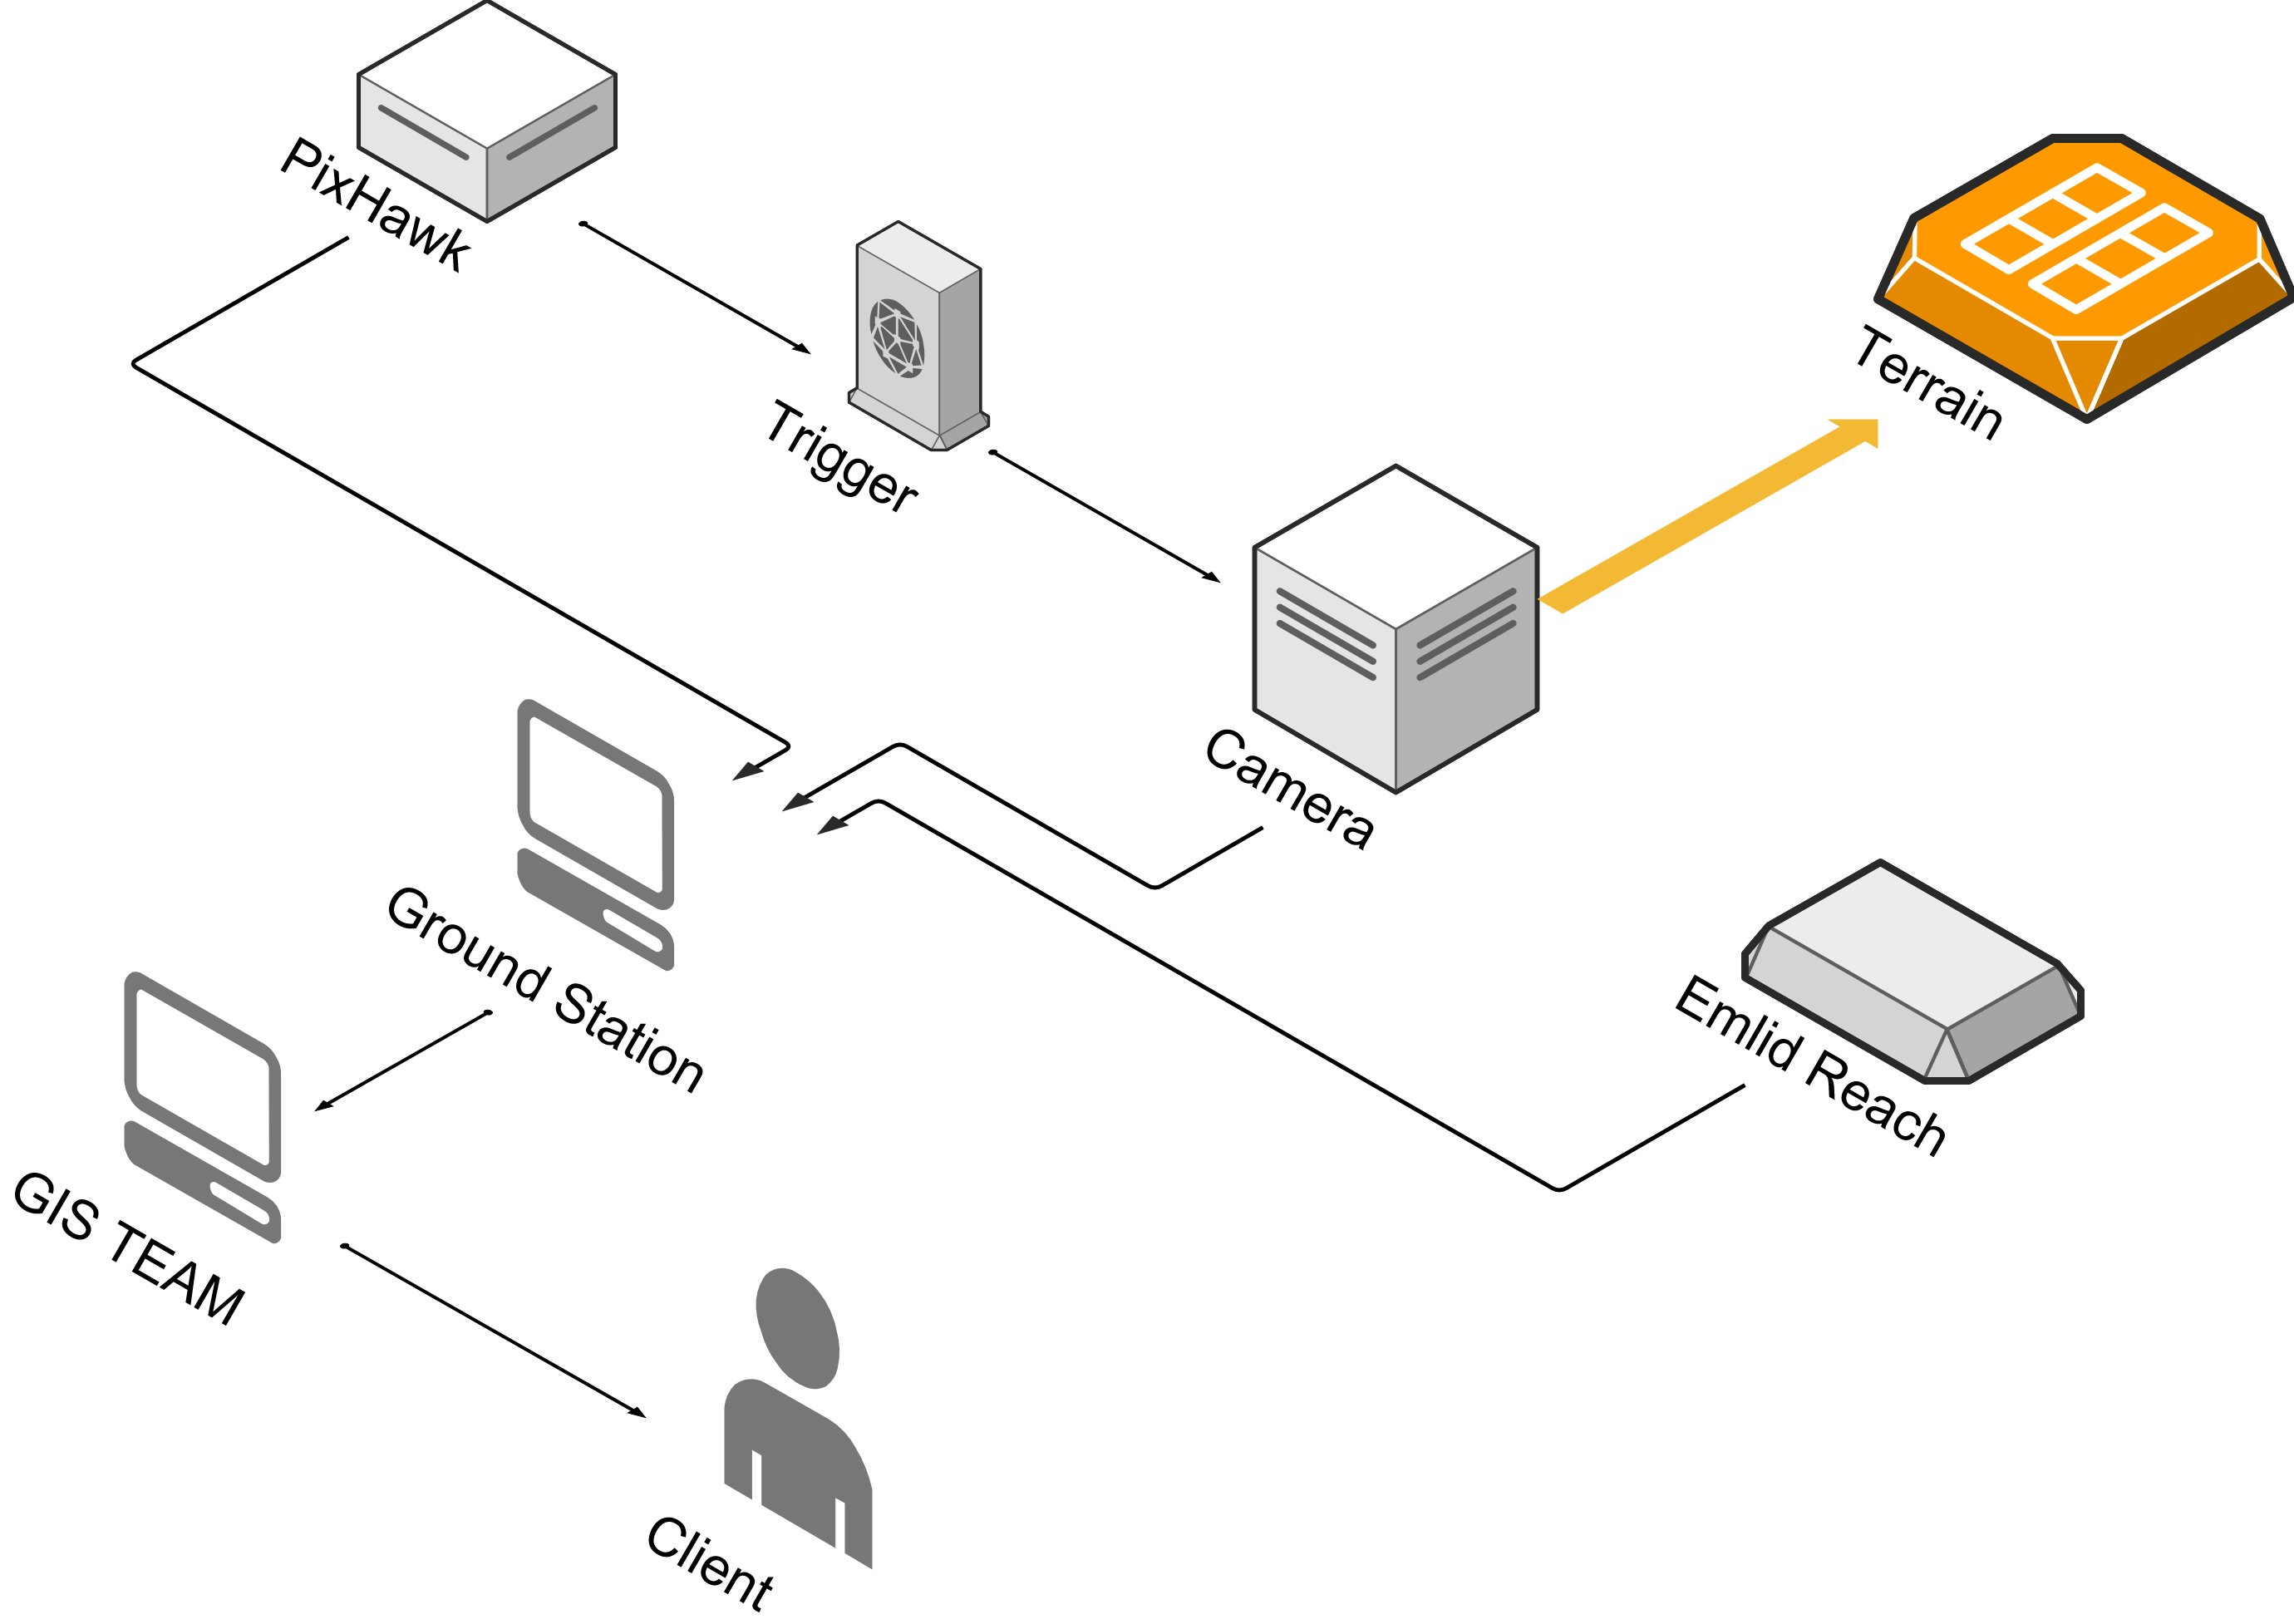
\includegraphics[width=\linewidth]{Present_System.jpg}
\\
The above is a representation of the present mode of operation we are using where the black connections represent the wired connections and the flow of data among objects.

\section{Explanation}
The flow of data is simple yet complicated because there are un automated transfers occuring which require humans to extract data individually and store in ground station. These need to be removed.
\\
\\
Here is the unautomated transfers shown
\\
\\
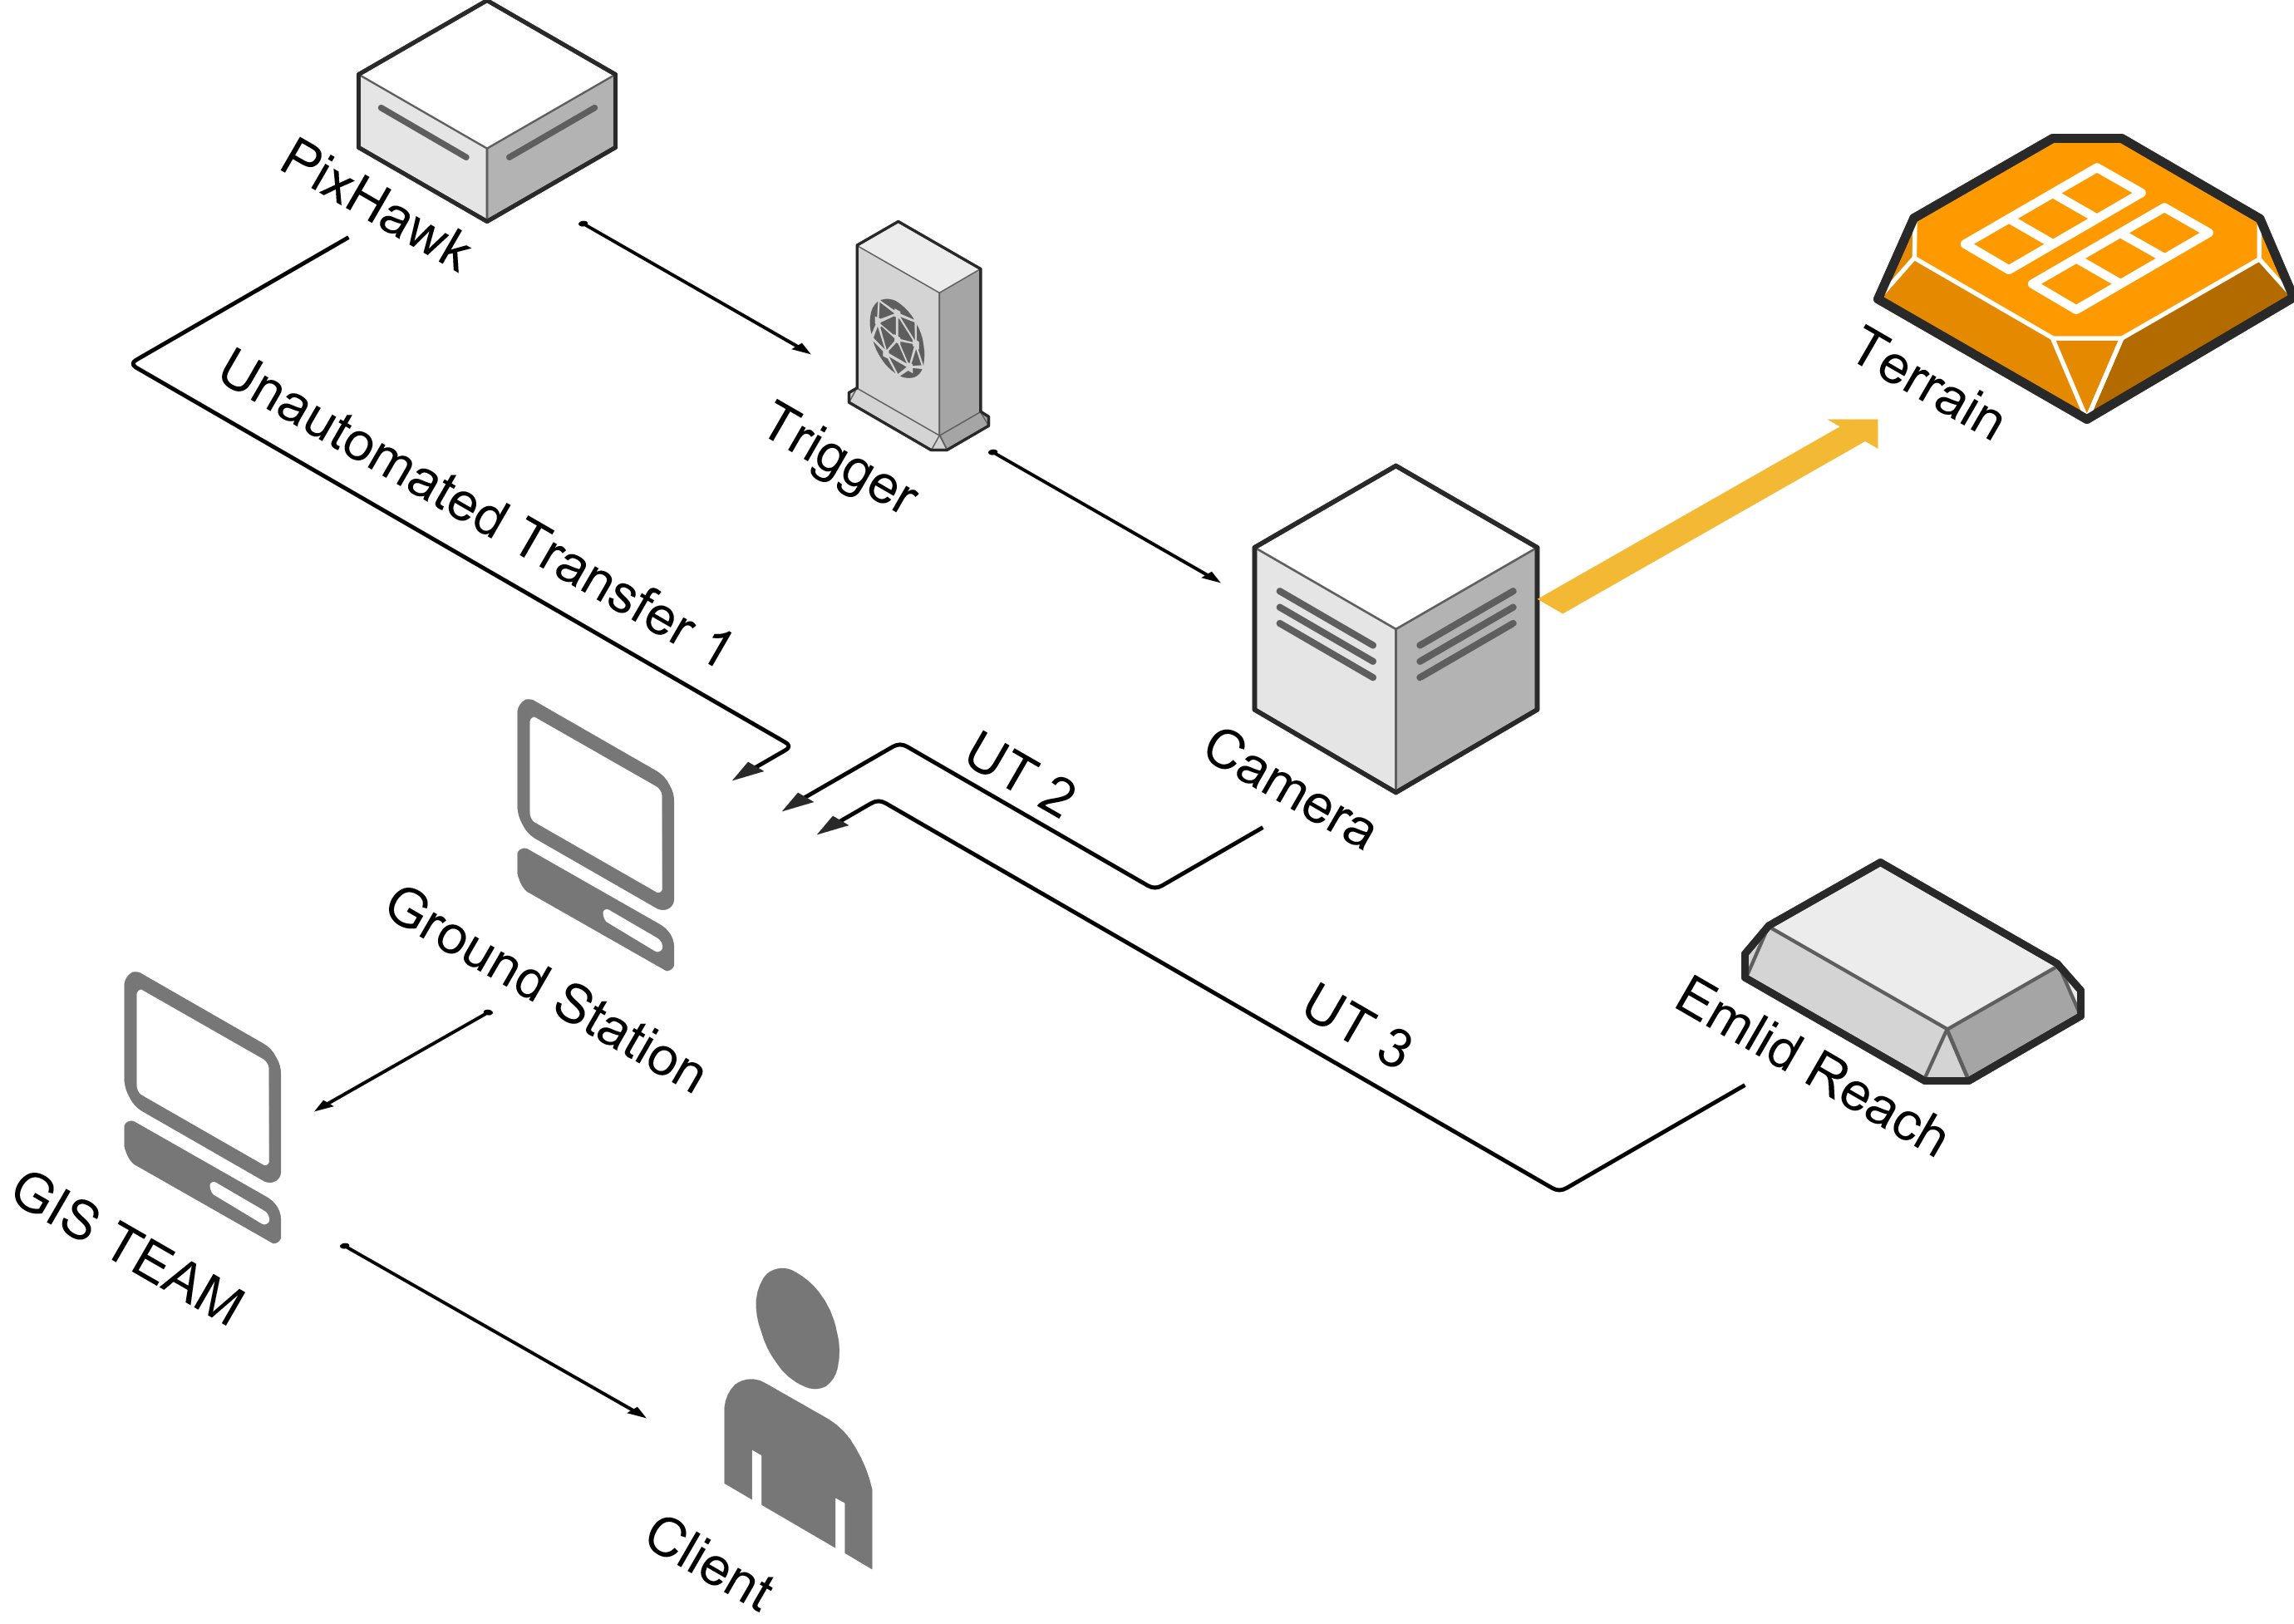
\includegraphics[width=\linewidth]{Present_Unautomated_System.jpg}
\\
\\
\begin{itemize}
\item UT 1 is presently via SD card or MAVLink
\item UT 2 is via SD card
\item UT 3 is via WiFi
\end{itemize}

\chapter{PixHawk 1 to PixHawk 2.1}
\section{Comparison}
PixHawk 2.1 can be explained better with the inclusion of this comparison chart:- 
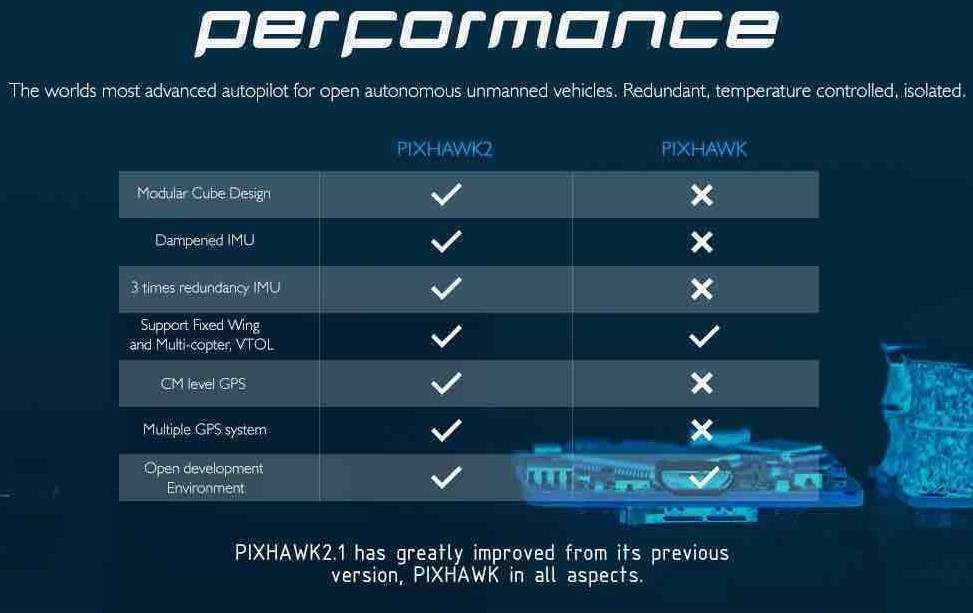
\includegraphics[width=\linewidth]{pixhawk2vs1.jpg}

\section{The HW differences}
This is due to the CUBE which is placed in between the breakout board of the PixHawk 2. This brain of the equipment contains separated IMU and FMU sensors. There is a layer of foam which resists high frequency vibration and thus reducing noise to the sensors. The cube also houses triple IMU system, composed of 3 accelerometers, 3 gyroscopes, 3 magnetometers, and 2 barometers. Most important of all, PixHawk 2 gives you a parallel computer slot. 


\chapter{The Intel Edison}
\section{Possibilities} 
 Imagine you are given a computer along with the PixHawk, flying online you can do a lot of computing. Here we will introduce  a few features that the Intel Edison features,
 \begin{itemize}
 \item Wifi telemetry to the autopilot
 \item Easy scripting/vehicle control via DroneKit
 \item Faster download of log files (coming soon)
 \end{itemize}

\section{Specefications}
 With overall
approximate dimensions of 34.9 × 25.4 × 3.2 mm. Under the metal cover is an Intel dualcore
Silvermont Atom processor running at a 500-MHz clock speed. There is also a 100-
MHz clocked Quark coprocessor included, which is designed to assist the Atom processor
with input/output (I/O) operations. Unfortunately, as of the time of this writing, Intel has
not released any software that will support the Quark coprocessor.

There is also 4 GB of flash memory and 1 GB of RAM available to support the internal
Edison processors. The flash memory comes preprogrammed with a Linux distribution
created by Intel engineers using the Yocto framework.

There is also a Broadcom BCM43340 chip contained in the module, which implements
b/g/n (11 Mbit/s, 56 Mbit/s, 100 Mbit/s internet speeds) and direct WiFi, as well as
Bluetooth Low Energy (BLE) wireless communication. Both the WiFi and Bluetooth (BT)
connections share the same onboard PCB chip antenna, which is visible at the lower lefthand
corner.

 An external antenna connector using a μFL standard format is
located just above the chip antenna and should be used if extended-range radio frequency
(RF) operations are required. The internal chip antenna is fairly limited and will likely
operate reliably only within 10 meters (m) of the WiFi access point, which is typically the
wireless router in most home networks. Of course, BT communications was always
designed to be close range, or not to exceed 10 m. One more point that you should know is
that the antenna (internal or external) is multiplexed, or shared, between WiFi and BT
operations. This might become problematic if maximum data bandwidth operations are
attempted using both modes simultaneously.

The Broadcom chip also supports a hardware WiFi access-point (AP) mode, which
might be very useful in certain applications. The only provision is that the module
software must also support this type of operation. Fortunately, the default Linux
distribution supports the AP mode, which allows for significant flexibility in configuring a
network containing the Edison. Intel also provided support for BlueZ 5.0, which
implements all the important and widely used BT profiles.

It
is a 70-pin connector manufactured by the Hirose company. It is considered high density
because of the very tight spacing between the connector pins, which are 35 pins spread
across 14 mm with 0.4 mm between pins. To put this in a common perspective, most
hobbyist’s solderless breadboards have a 0.1-inch, or 2.54-mm, spacing between insertion
points. The contacts on the Hirose connector are about six times closer than those on a
breadboard. The practical meaning for this situation is that the Edison can be used only
with a development board with the matching male connector already installed on a PCB. It
is just not feasible to manually solder 70 wires to a freestanding male Hirose 70-pin
connector.

\section{Shortcomings} 
It might be possible to solder a few wires to such a connector, using a
magnifying lens and an extremely sharp-pointed soldering iron, but I think it is beyond my
skill level as well as that of most of my readers. \emph{Another point worth mentioning is that Hirose connector was not designed to be inserted and removed frequently. You can do operations a few times, but be very careful as it is easy to damage the connecting by misaligning them and/or using excessive force}. I believe this will not be an issue
for most readers, as they likely will just mount the Edison on an appropriate development
board and simply use the board with their projects.

 Edison has 40 general-purpose input/output
(GPIO) pins that are available in the Hirose connector, in addition to the dedicated pins
used for power and communications, but once it goes into the PixHawk 2.1 it will be very difficult to make use of all the pins, as the PH 2.1 is like a small coffin for the IE making only 2 ports via USB available for the Edison.

\chapter{Camera}
\section{Specifications}
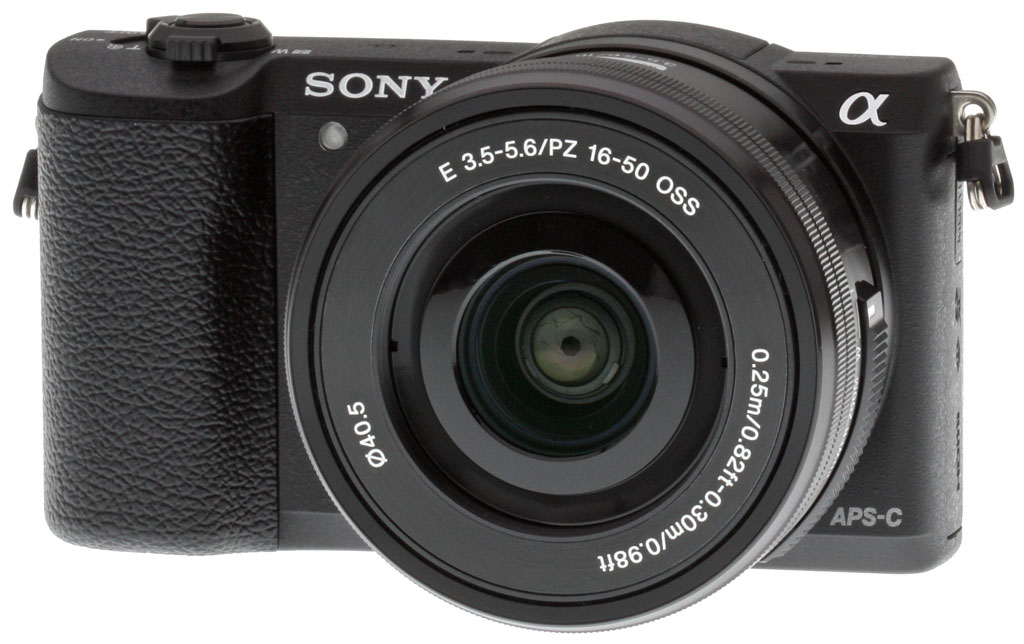
\includegraphics[width=\linewidth]{Camera.jpg}
\\
The camera being used in the present setup is a Sony $\alpha$ 5100 series camera and it has a lot to offer as follows:-
\\
\newpage
General
\\
Model Number:
A5100
\\Alternate Model Number(s):
ILCE-5100
\\Camera Format:
Compact System Camera
\\Currently Manufactured:
Yes
\\Retail Price:
~Rs. 45,000
\\Date Available:
2014-09-01
\\Tripod Mount:
Yes
\\Weight:
14.1 oz (399 g) 
includes batteries, kit lens 
\\Size:
4.3 x 2.5 x 1.4 in.
(110 x 63 x 36 mm) 
\\Waterproof:
No
\\Waterproof Depth:
n/a
\\  \\Image Sensor
\\Sensor Type:
CMOS
\\Sensor Manufacturer:
Sony
\\Effective Megapixels:
24.3
\\Sensor Format:
APS-C
\\Sensor size:
366.6mm2 (23.50mm x 15.60mm)
\\Approximate Pixel Pitch:
3.92 microns
\\Focal Length Multiplier:
1.5x
\\Aspect Ratio:
3:2 
\\Color Filter Type:
RGBG
\\Anti Aliasing Filter:
Fixed
\\Self-Cleaning:
No
\\Sensor shift image stabilization:
No
\\On-Sensor Phase Detect:
Yes
\\DxO Sensor Score:
80
\\DxO Color Depth Score (bits):
23.8
\\DxO Dynamic Range Score (evs):
12.7
\\DxO Maximum Effective ISO Score (iso):
1,347
\\  \\Image Capture
\\Image Resolution:
6000 x 4000 (24.0 MP, 3:2),
6000 x 3376 (20.3 MP, 16:9),
4240 x 2832 (12.0 MP, 3:2),
4240 x 2400 (10.2 MP, Other),
3008 x 2000 (6.0 MP, 3:2),
3008 x 1688 (5.1 MP, 16:9),
12416 x 1856 (23.0 MP, Other),
8192 x 1856 (15.2 MP, Other),
2160 x 5536 (12.0 MP, Other),
2160 x 3872 (8.4 MP, Other) 
\\Image File Format:
JPEG (EXIF 2.3), RAW (ARW 2.3), RAW+JPEG 
\\Continuous-mode frames/second:
6.0
\\  \\Video Capture
\\Can take movies:
Yes
\\Movie Resolution:
1920x1080 (60p/60i/30p/24p) 
1440x1080 (30p) 
640x480 (30p) 
\\Movie File Format:
XAVC S / AVCHD 2.0 / MP4; \\Stereo Audio: Dolby Digital (AC-3) / MPEG-4 AAC-LC
\\Composite Video Out:
No
\\NTSC/PAL Switchable Video:
n/a
\\Video Usable as Viewfinder:
n/a
\\HD Video Out:
Yes
\\HD Video Connection:
HDMI
\\  \\Lens and Optics
\\Lens Mount:
Sony E
\\Lens:
Sony SELP1650 PZ 16-50mm f/3.5-5.6 OSS; 9 elements in 8 groups, 4 aspheric surfaces
\\Focal Length (35mm equivalent):
24 - 75mm 
\\Focal Length (actual):
16 - 50mm 
\\Zoom Ratio:
3.13x
\\Aperture Range:
f/3.5 - f/22 (W) / f/5.6 - f/36 (T); 7-blade circular aperture
\\Integrated ND Filter:
No
\\Normal Focus Range:
25 cm to Infinity
9.8 in to Infinity 
\\Macro Focus Range:
\\Filter Thread:
40.5mm
\\Thread Type:
n/a
\\Optical Image Stabilization:
Yes
\\Digital Zoom:
Yes
\\Digital Zoom Values:
Up to 4x; up to 2x Clear Image Digital Zoom
\\  \\Auto Focus
\\Auto Focus:
Yes
\\Auto Focus Type:
Hybrid Contrast/Phase Detection: 179-point PDAF, 25-point CDAF, Center, Flexible Spot (S/M/L), Zone
\\Auto Focus Assist Light?
Yes
\\Manual Focus:
Yes
\\  \\Viewfinder
\\Viewfinder:
No / LCD 
\\Viewfinder Type:
\\Focus Peaking:
Yes
\\EVF Resolution:
n/a 
\\Viewfinder Magnification (35mm equivalent):
\\Viewfinder Magnification (nominal/claimed):
\\  \\Display
\\Eye-level Viewfinder:
No
\\Rear Display:
Yes
\\Rear Display Size (inches):
3.0
\\Rear Display Resolution:
921,600 dots (230,400 px) 
\\Touchscreen:
Yes
\\Articulating Screen:
Yes
\\Tilt Swivel Screen:
No
\\Selfie Screen:
Yes
\\Max Playback Zoom:
16.7x
\\Top Deck Display:
No
\\Exposure
\\Maximum ISO (native):
25600
\\Minimum ISO (native):
100
\\ISO Settings:
Auto, 100, 200, 400, 800, 1600, 3200, 6400, 12800, 25600
\\Auto ISO Mode:
Yes
\\White Balance Settings:
Auto WB, Daylight, Shade, Cloudy, Incandescent, Fluorescent (Warm white/Cool white/Day white/Daylight), Flash, Underwater, C. Temp 2500 to 9900K, C Filter G7 to M7 (15-step), Custom, AWB micro adjustment
\\Shutter Speed Range:
30 - 1/4000
\\Bulb Mode:
Yes
\\Exposure Compensation:
+/- 3.0EV in 0.3EV steps 
\\Metering Modes:
1200-zone Evaluative, Center-weighted, Spot
\\Program Auto Exposure:
Yes
\\Aperture Priority:
Yes
\\Shutter Priority:
Yes
\\Full Manual Exposure:
Yes
\\Creative Exposure Modes:
Portrait, Landscape, Macro, Sports Action, Sunset, Night Portrait, Night Scene, Hand-held Twilight, Anti Motion Blur, HDR, Sweep Panorama
\\Self Timer:
2 , 10, 10 (3 or 5 frames) seconds
\\Time Lapse (intervalometer):
\\High Resolution Composite:
No
Flash
\\Built-in Flash:
Yes
\\Flash Modes:
Auto, Off, Fill-flash, Rear sync, Slow sync, Red-eye reduction: On/Off
\\Flash Guide Number (ISO 100):
4.0 m / 13.1 ft. 
\\Flash Range Description:
Lens dependent; GN=4 (ISO 100, m)
\\Max Flash Sync:
1/160
\\Flash Exposure Compensation:
+/- 2.0 EV in 0.3EV steps 
\\External Flash Connection:
n/a
\\Built-In Wireless Flash Control:
No
\\  \\Image Storage
\\Usable Memory Types:
MS PRO Duo / SD / SDHC / SDXC
\\UHS Support:
UHS-I
\\Other Memory:
\\Dual Card Slots:
No
\\RAW Capture Support:
Yes
\\Uncompressed Format:
RAW (ARW 2.3), RAW+JPEG
\\Movie File Format:
XAVC S / AVCHD 2.0 / MP4; Stereo Audio: Dolby Digital (AC-3) / MPEG-4 AAC-LC
\\Included Memory:
No memory included
\\Included Memory Type:
\\ \\Connectivity
\\Built-In Wi-Fi:
Yes
\\NFC:
Yes
\\Bluetooth:
No
\\Built-In GPS:
No
\\Microphone Jack:
No
\\Headphone Jack:
No
\\External Connections:
USB 2.0 High Speed,WiFi
\\PictBridge Compliant:
Yes
\\DPOF Compliant:
Yes
\\Remote Control:
Yes
\\Remote Control Type:
Optional wired or Wi-Fi
\\Connections (extended):
Micro (Type-D) HDMI, Multi Micro USB
Performance Timing
\\Cycle time for JPEG shooting in single shot mode (seconds per frame, max resolution):
0.55
\\Cycle time for RAW shooting in single shot mode (seconds per frame):
0.59
\\Buffer size for RAW shooting in single shot mode (frames):
Unlimited
\\Cycle time for RAW+JPEG shooting in single shot mode (seconds per shot):
0.56
\\Camera penalizes early shutter press?
No
\\JPEG shooting speed in burst mode (fps, max resolution):
6.0
\\Buffer size for JPEG shooting in burst mode (frames, max resolution):
67
\\RAW shooting speed in burst mode (fps):
6.0
\\Buffer size for RAW shooting in burst mode (frames):
25
\\RAW+JPEG shooting speed in burst mode (fps):
6.0
\\Buffer Size for RAW+JPEG shooting in burst mode (frames):
23
\\Shutter lag (full AF, wide/mid):
0.24 seconds
\\Shutter lag (full AF, tele):
\\Shutter lag (full AF, live view - DSLR):
\\Shutter lag (prefocused, live view - DSLR):
\\Shutter Lag (manual focus):
0.126 seconds
\\Shutter lag (full AF, with flash):
0.35 seconds
\\Shutter Lag (prefocused):
0.021 seconds
\\Shutter Lag (notes):
Full AF shutter lag, wide-area AF mode = 0.230s
\\Startup Time:
2.0 seconds
\\Play -> Record Time:
1.0 seconds
\\Flash cycle time, full power:
2.2 seconds
Power
\\Battery Life, Stills (CIPA Rating Monitor/Live View):
400 shots 
\\Battery Life, Still (CIPA Rating OVF/EVF):
\\Battery Life, Video:
\\Battery Form Factor:
Proprietary NP-FW50
\\Usable Battery Types:
Lithium-ion rechargeable
\\Batteries Included:
1 x Proprietary NP-FW50 Lithium-ion rechargeable 
\\Battery Charger Included (dedicated charger or AC/USB adapter):
Yes
\\Dedicated Battery Charger Included:
No
\\Internal Charging Supported:
Yes
\\  \\Software
\\Included Software:
Sony Play Memories is a pre requisite for communicating via any way with other devices. 
\\OS Compatibility:
Windows and Mac OS

\section{The Problem and solution}
As you will see ahead in the solution section  you will see with the entry of Intel Edison into the scenario we see the camera has connections with the trigger as well as the Intel Edison. However the problem which we face in this type of arrangement is that there is only one micro-USB B type port on the camera which needs connection with both. Also if we just provide a port of superimposed trigger multiport and the data transfer micro USB from Intel Edison to the Camera, the camera somehow enters USB mass storage mode rendering it useless for image capture. Thus there is a need to multiplex between the USB transfer mode and the capture mode.
\\
\\
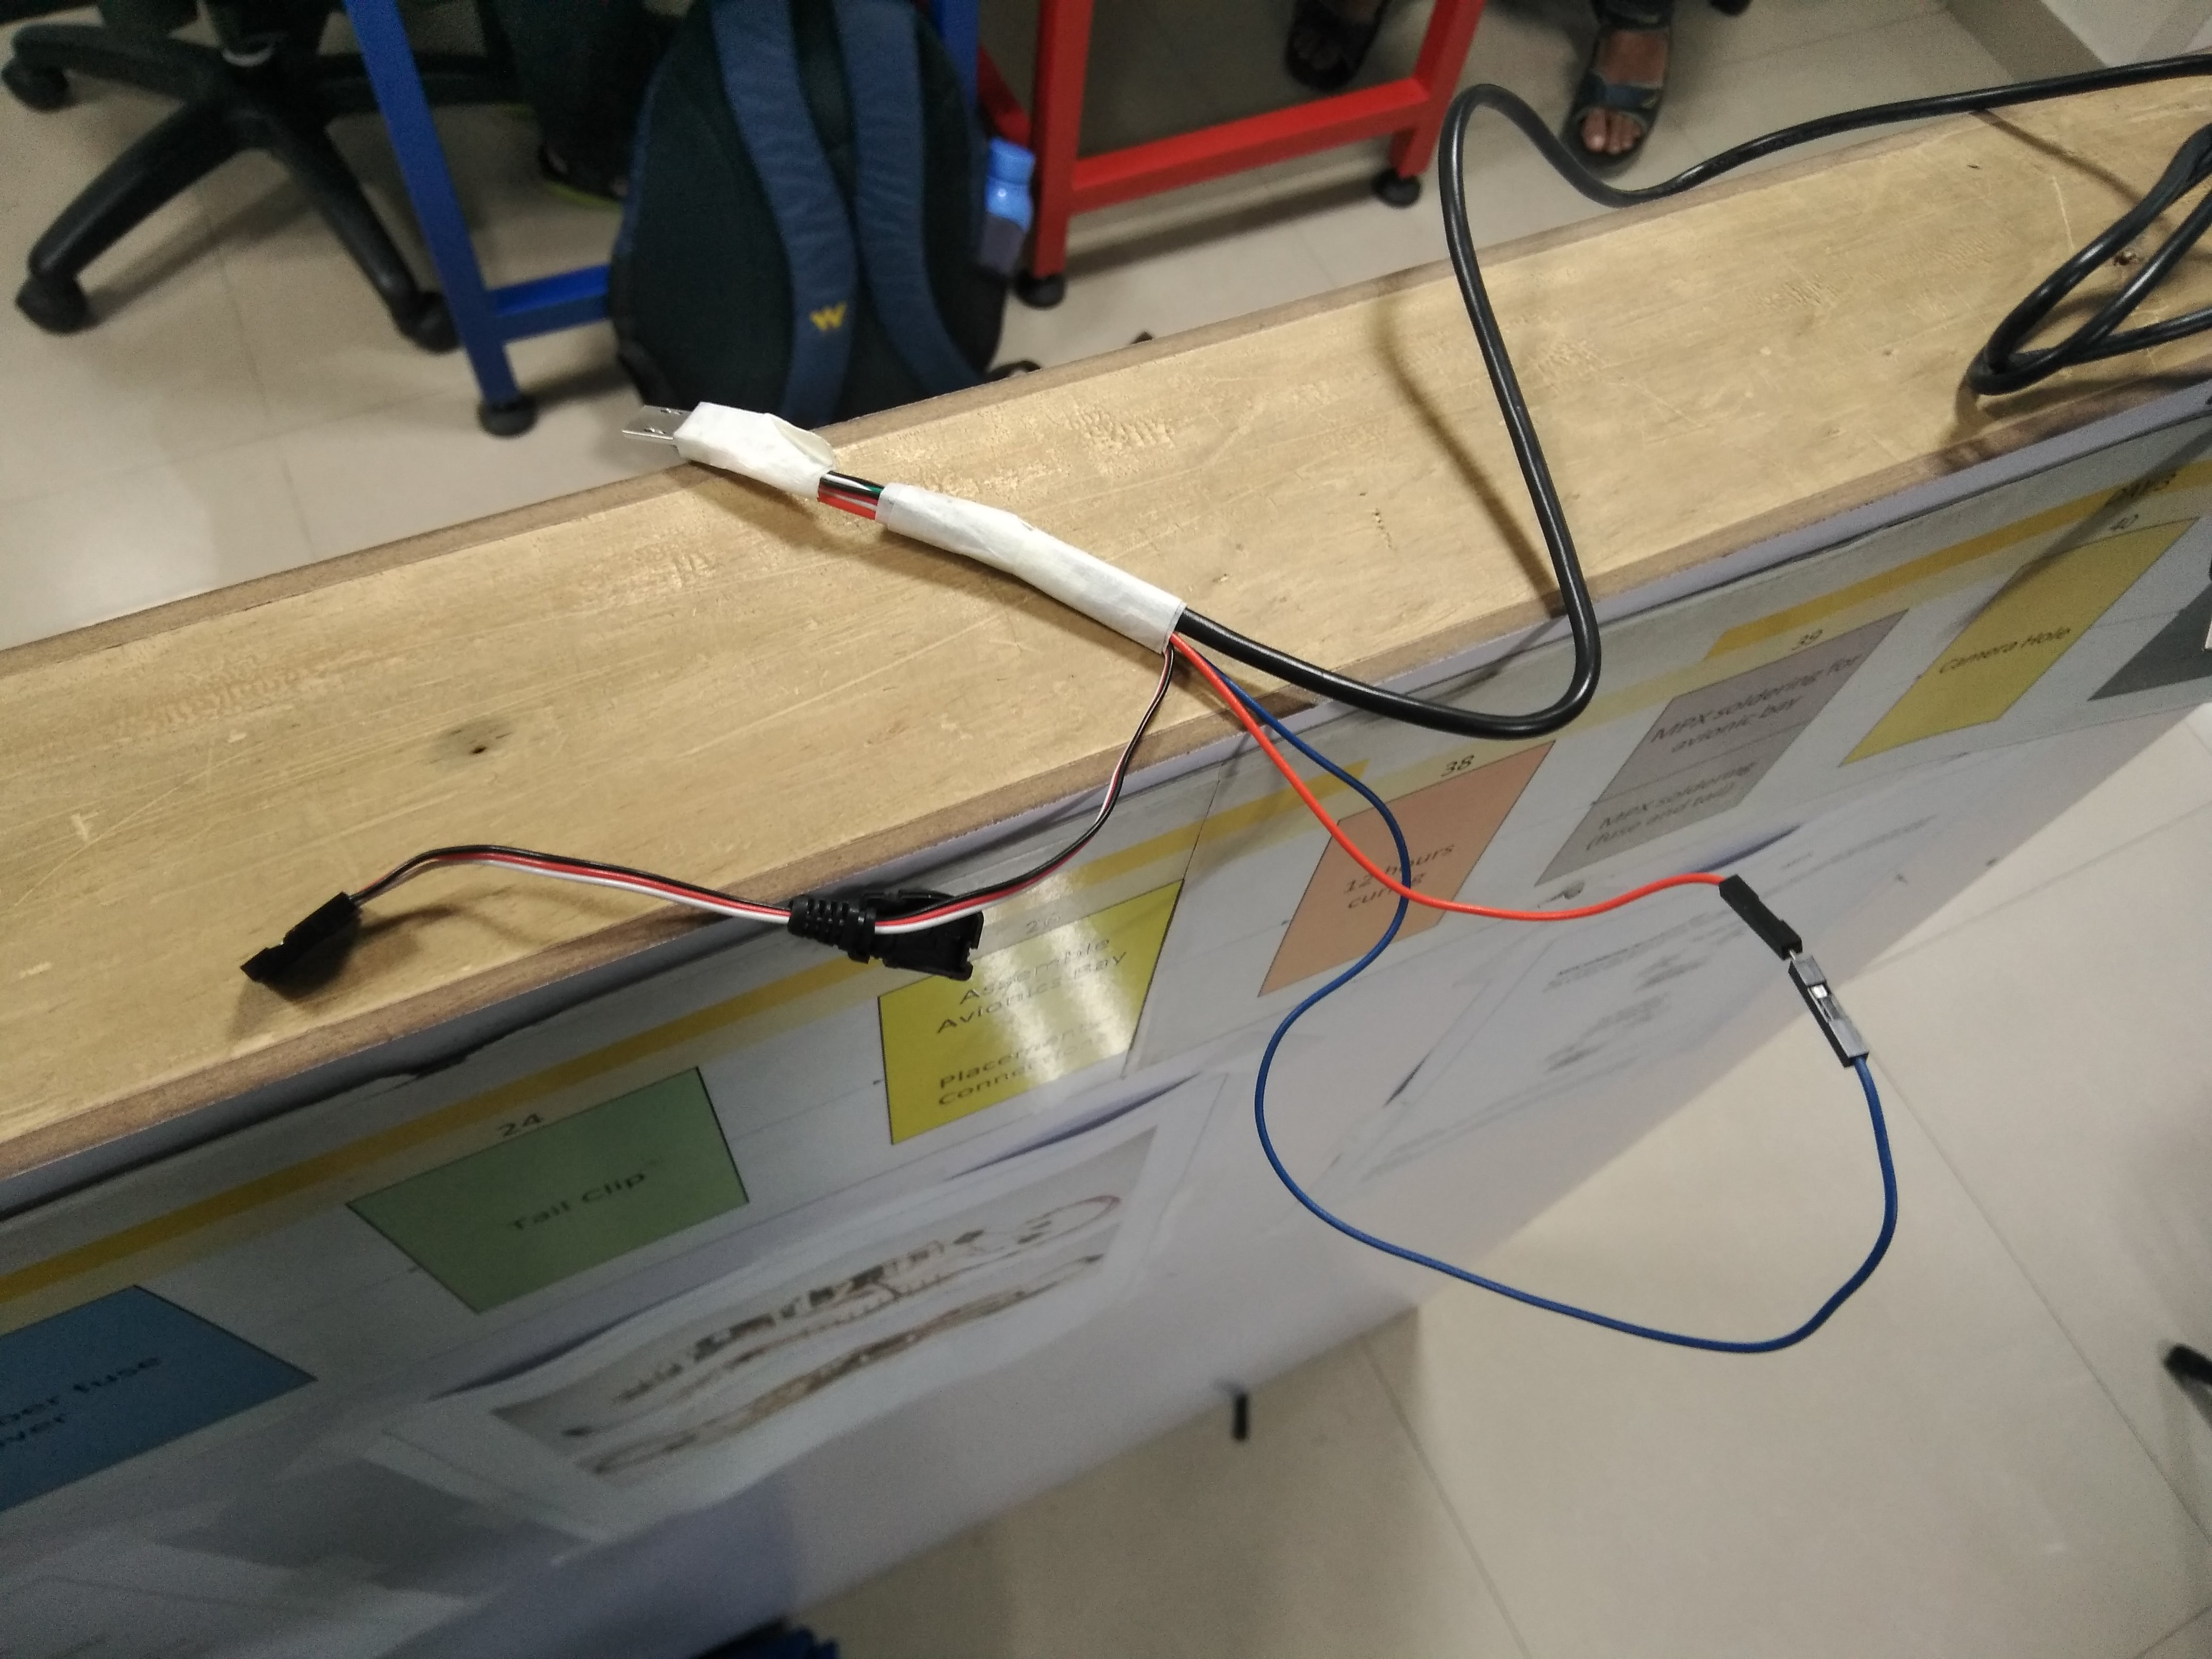
\includegraphics[width=\linewidth]{Camera_USB.jpg}
\\ \\
The above figure is a solution which we processed at the DroneCubator section, this is superimposition of a multi-port trigger for the camera and the data transfer USB. The blue-red jumper connections are the key to switch modes. The blue-red line shouldn't be connected anytime during the flight, i.e. the capture mode is when those two are not connected. However once both are connected USB transfer can occur.
\\
\\
A library named "gphoto2" can be used to conduct mass file transfer operations.

\chapter{Emlid Reach}
\section{RTKLIB}
RTKLIB is an amazingly powerful open-source software written by Tomoji Tokasu for RTK and postprocessing. Algorithms used to determine accurate position are computational intensive and RTKLIB was mostly used on PCs and laptops. We have created a tiny, yet very powerful module that runs RTKLIB and locates your position with centimeter precision.

\section{9DOF}
Knowing precise position is not always enough, Reach packs an inertial measurement unit with 3-axis gyroscope, 3-axis accelerometer and 3-axis magnetometer. This opens new possibilities for orientation estimation and for fusion with GPS data. In the future we will be able to improve positioning accuracy using the IMU

\section{Edison Inside}
Powered by Intel Edison Reach is truly an internet of things device. Wi-fi and Bluetooth 4.0 connectivity is already built-in, allowing for easy communication to your smartphone, tablet or cloud. And when there is no Wi-fi hotspot nearby USB OTG will power LTE modem, though we do not use the 4G modem to communicate.

\section{Real Time Kinematics}
Main function of Reach is to compute precise coordinates. To do so it uses technology called RTK – Real-time kinematics. Two connected receivers within 10km radius are used and static device streams corrections to the moving one. You can simply connect one device to your home router and another one to a smartphone with web access.

\section{Problem Statement and Solution}
With the advent of this device successful integration of this has been done with the PixHawk onboard however post-processing requires the latest log file from the Emlid onboard. My work is on getting the file to ground station automatically.
 \\
 \\
We exploit the availability of the Intel Edison onboard to transfer the log files wireless-ly via SSHing into the terminal flying onboard. A script is written which will get the latest log file in the format 'raw*.UBX' to the ground station and make it available to Adnan's code for post-processing.
\\
\\
The GitHub link to the script is: \\ https://github.com/samvram/emlidautomation
\\ 
Here is the version of code as on 31/05/2017
\\
\begin{verbatim}
#!c:/Python/python.exe -u

# This block of code gets the latest file and stores it in the location 
#the script runs in


import base64

import paramiko

import cmd



# Creating a SSH client named 'client'

# The method is to bypass RSA SSH DNA key so the 2nd line does Auto Add

client = paramiko.SSHClient()

client.set_missing_host_key_policy(paramiko.AutoAddPolicy())   



# The IP is to be set a proper static one, 
#the given username and password are present for SSHing

client.connect('192.168.3.145', username='root', password='emlidreach')



#Initialization of lists that are essential for finding the latest file

sam=[];

raw=[];

dt=[];







# We get file list of logs, print it as well as store it in the list sam

stdin, stdout, stderr = client.exec_command('ls logs')

for line in stdout:

    print('>>> ' + line.strip('\n'))

    sam.append(line.strip('\n'))





# We filter to get the name of all raw files from sam and print all 
#file names

print('sam is:')

for i in range(0,len(sam)):

    print(sam[i])

    if(sam[i][0:3] == 'raw'):

        raw.append(sam[i])



# We print all the raw files and get the date and time part of
#the filename and add them to date list

print('\n The raw files are')

for i in range(0,len(raw)):

    print(raw[i])

    dt.append(raw[i][4:-4])



# dt is a string list and we make it integer while printing them

print('\n The dates are')

for i in range(0,len(dt)):

    dt[i]=int(dt[i])

    print(dt[i])



# We find the latest date as it is the largest value present

for i in range(0,len(dt)):

    if(max(dt)==dt[i]):

        latestfile=raw[i]



# Printing the name of the latest file

print('\nThe latest file is ',latestfile)

resultfile = latestfile



# Appending the complete address to get the files from

latestfile = 'logs/'+latestfile



#FTP Standard protocol commands to make file transfer

ftp = client.open_sftp()

ftp.get(latestfile,resultfile)

ftp.close()



print('\nThe result file has been saved\n')



client.close()
\end{verbatim}

\chapter{Possible Solution Networks}
\section{Alternate solution 1}
 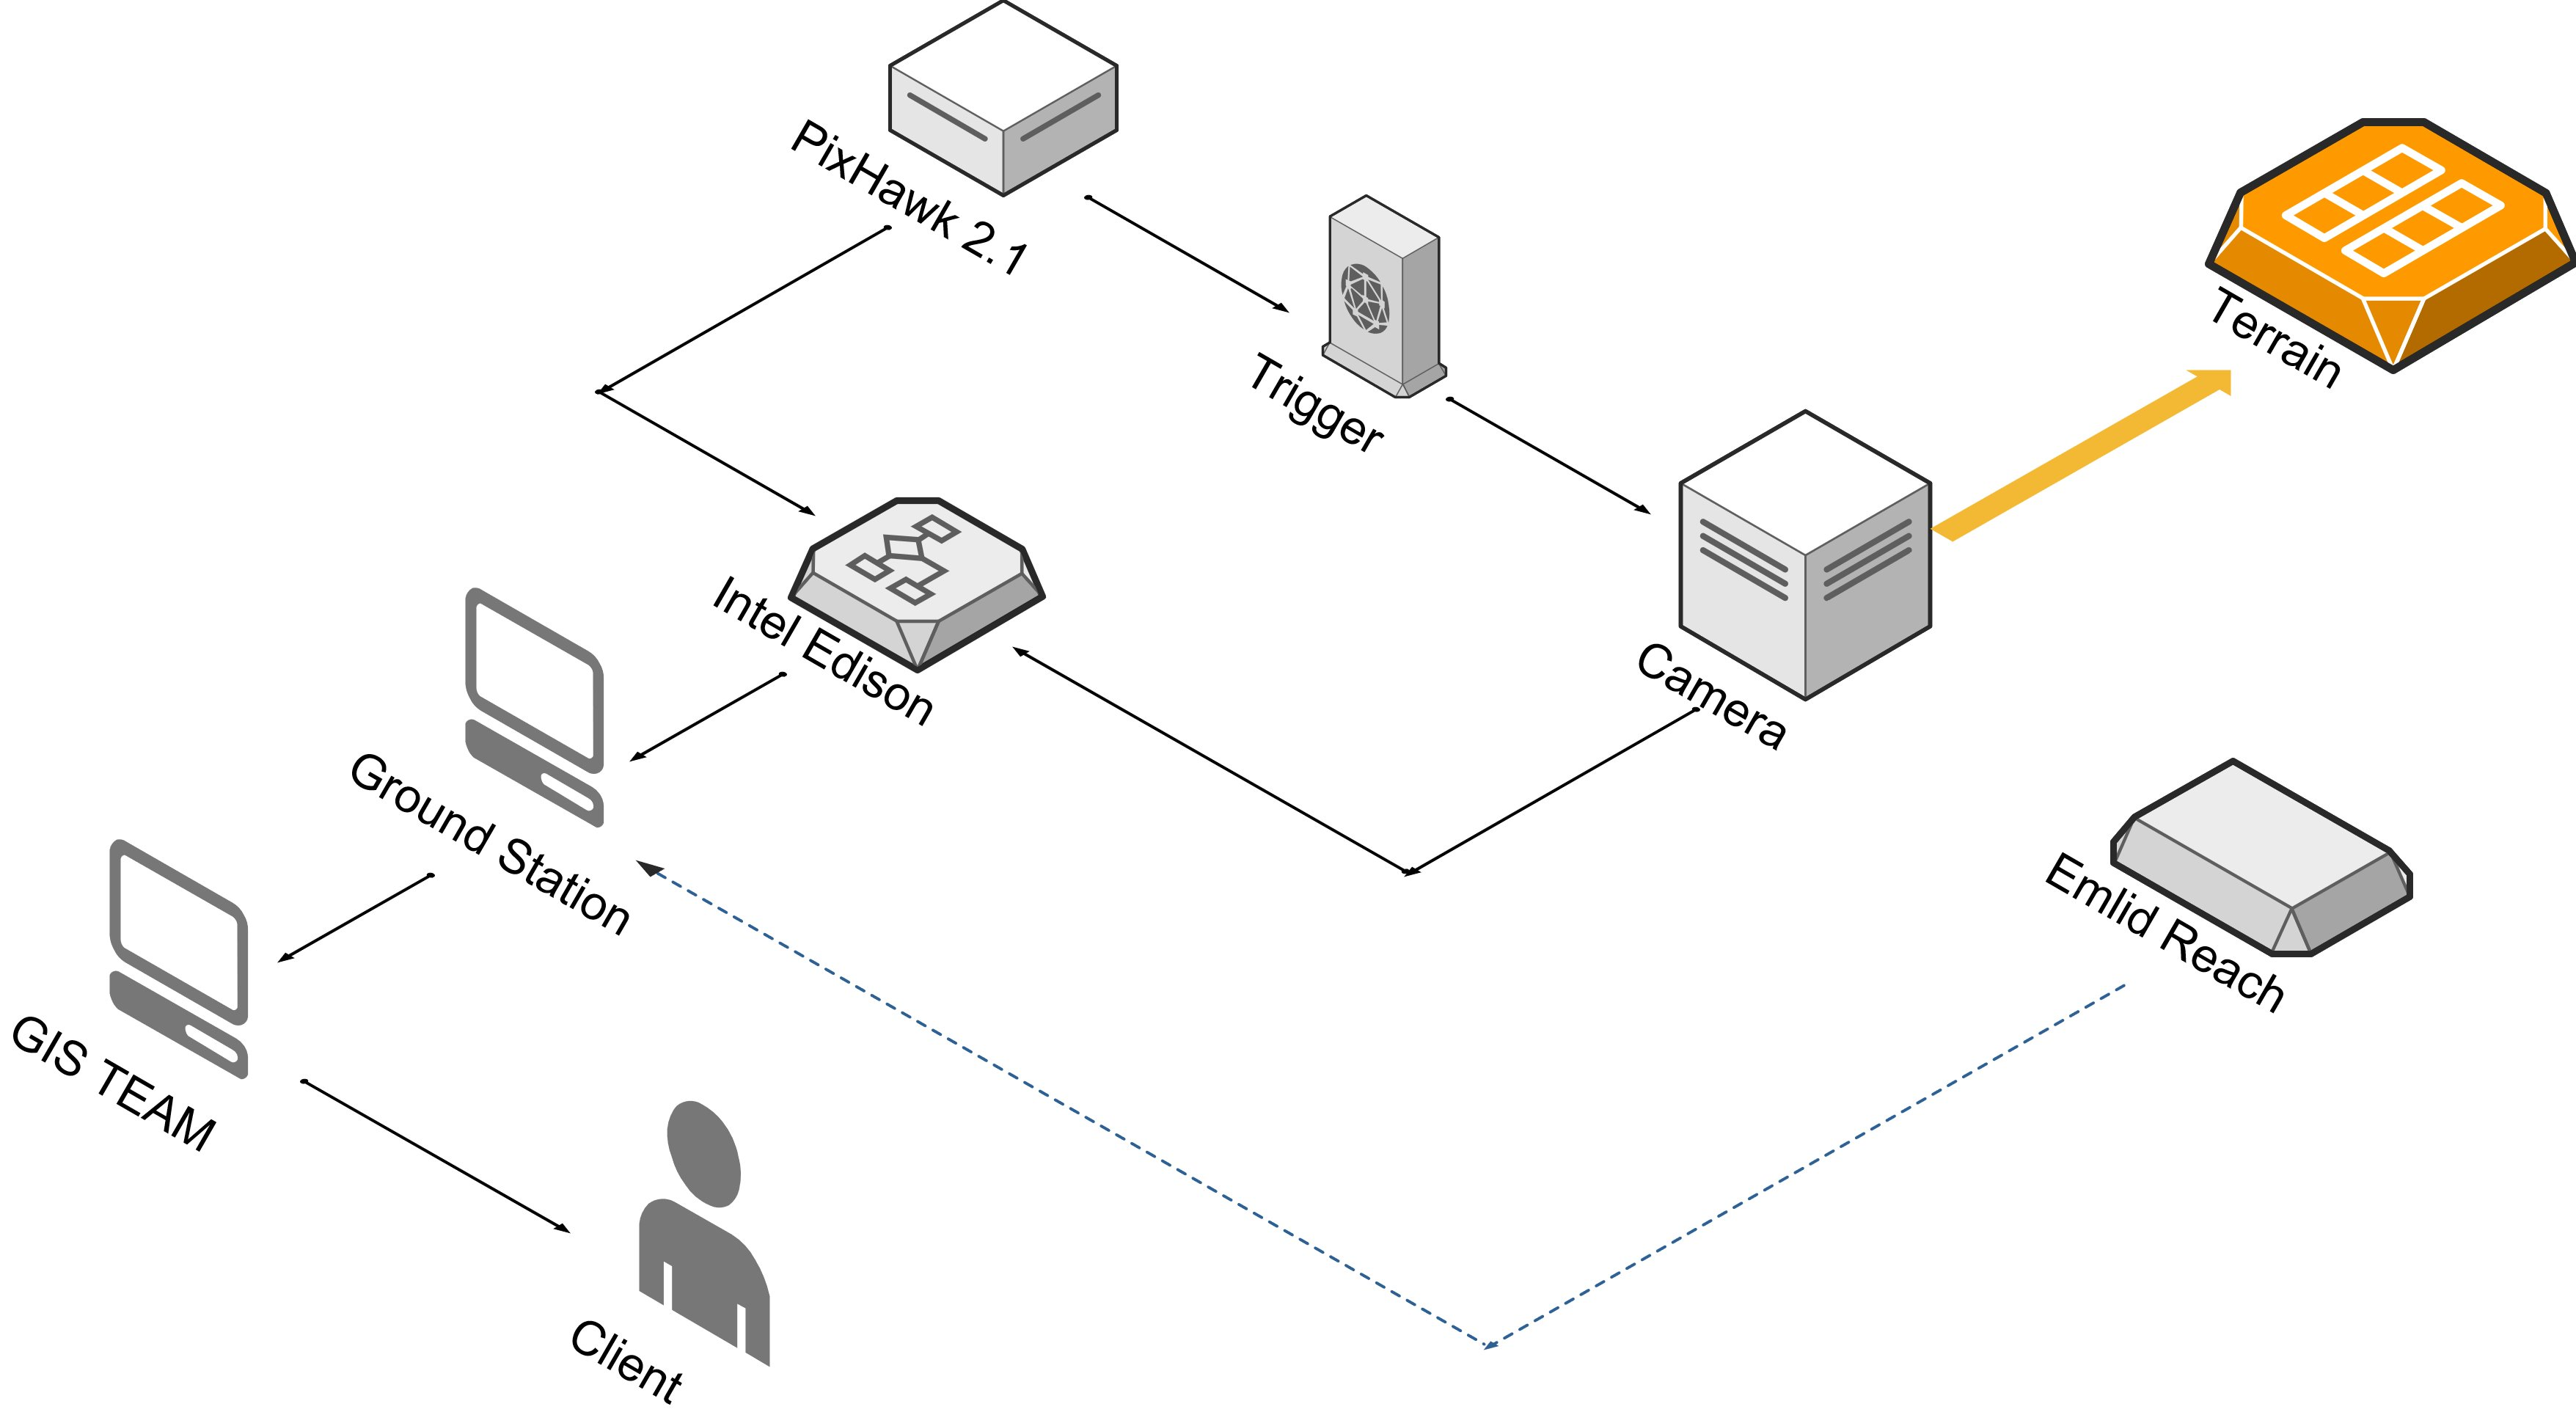
\includegraphics[width=\linewidth]{Alternative_Solution1.jpg}
\\
There is wired connection between all mostly except wireless transfer mechanism with the Emlid Reach.
\subsection{Advantages}
Due to the prevalent wired transfers the transfers are expected to occur at higher speeds contrary to wireless ones.
\subsection{Disadvantages} 
The ground-station has to get data from 3 sources, namely the Intel Edison of PixHawk 2.1 and both of the Emlids.
\section{Alternate solution 2}
 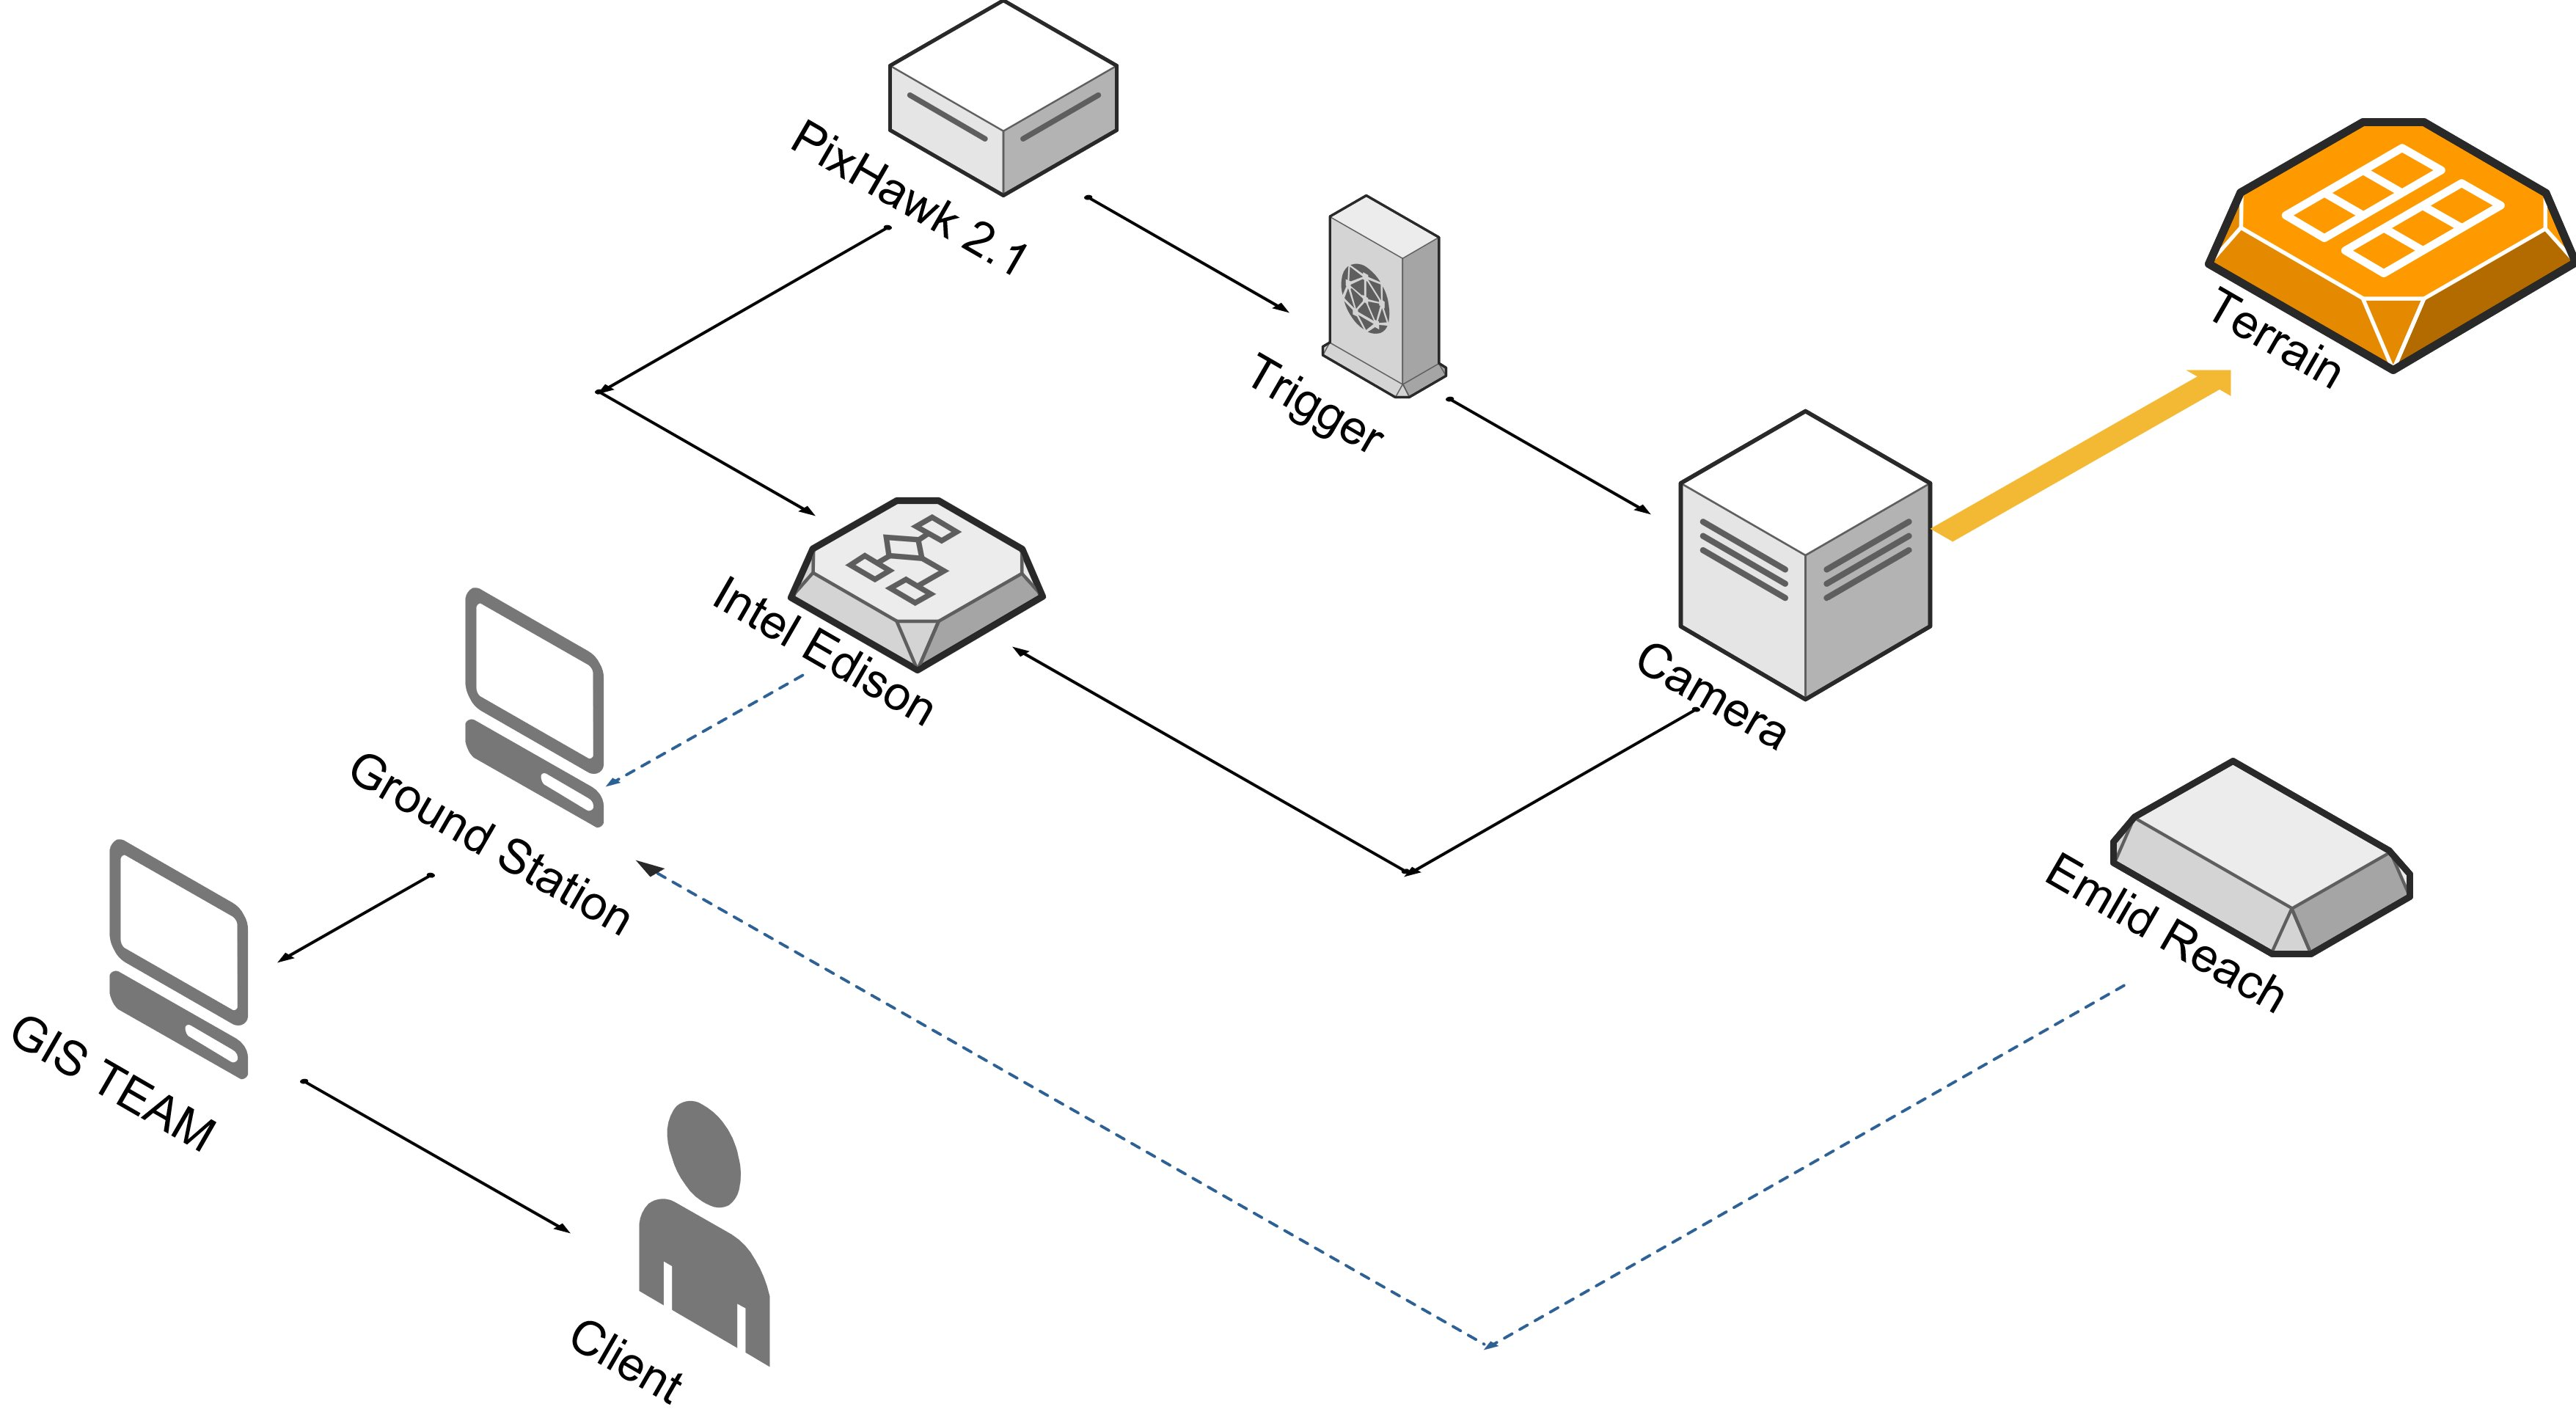
\includegraphics[width=\linewidth]{Alternative_Solution2.jpg}
 \\ 
 This is pretty much the same as the first solution but there is wireless transfer between Intel Edison of PixHawk 2.1 and the ground-station.
\subsection{Advantages}
There is no wired connection required with the ground-station, just that it should be inside the WiFi field region.
\subsection{Disadvantages} 
 Wireless transfer of large amounts of data can be very very slow leading to system failures.
 
\section{Alternate solution 3}
 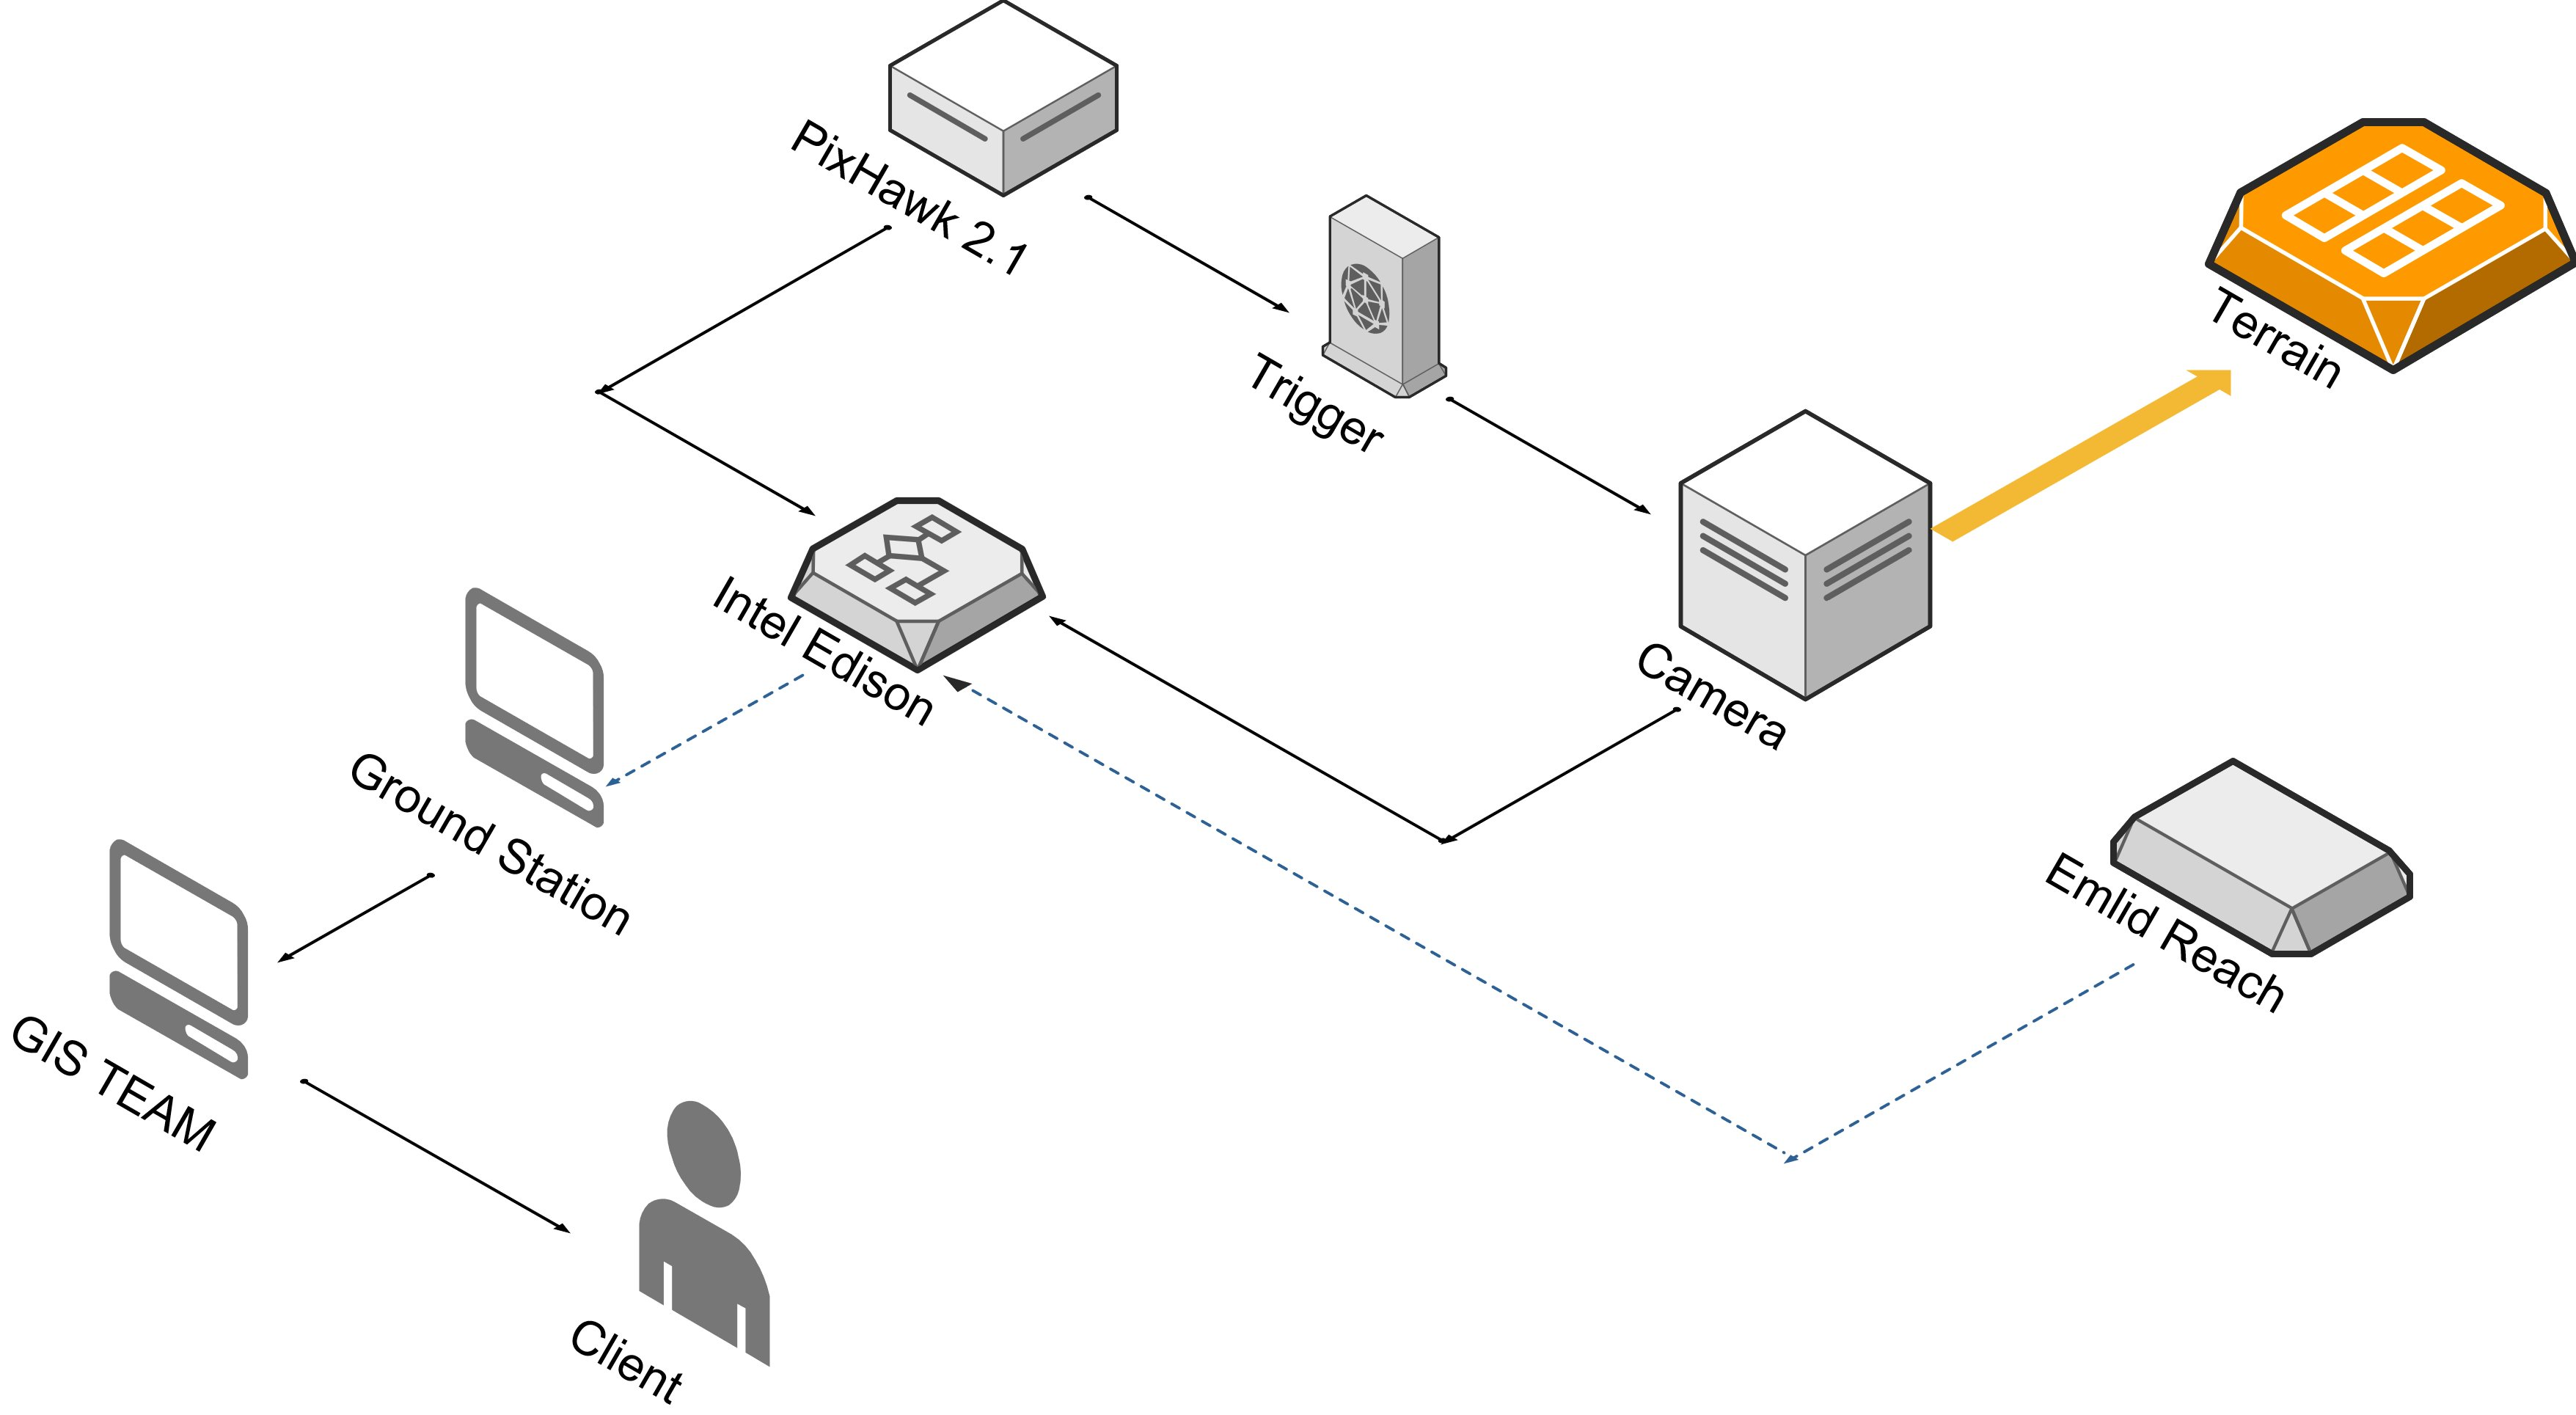
\includegraphics[width=\linewidth]{Alternative_Solution3.jpg} 
  \\ 
 This is similar to the previous solution except that the ground-station communicates to only one Intel Edison via \emph{wireless} communication.
\subsection{Advantages}
Since communication channel is centralized it will require a simpler implementation on the DMC.
\subsection{Disadvantages} 
  There is wireless transfer between Ground-station and the Intel Edison thus  making it slow.

\section{Alternate solution 4}
 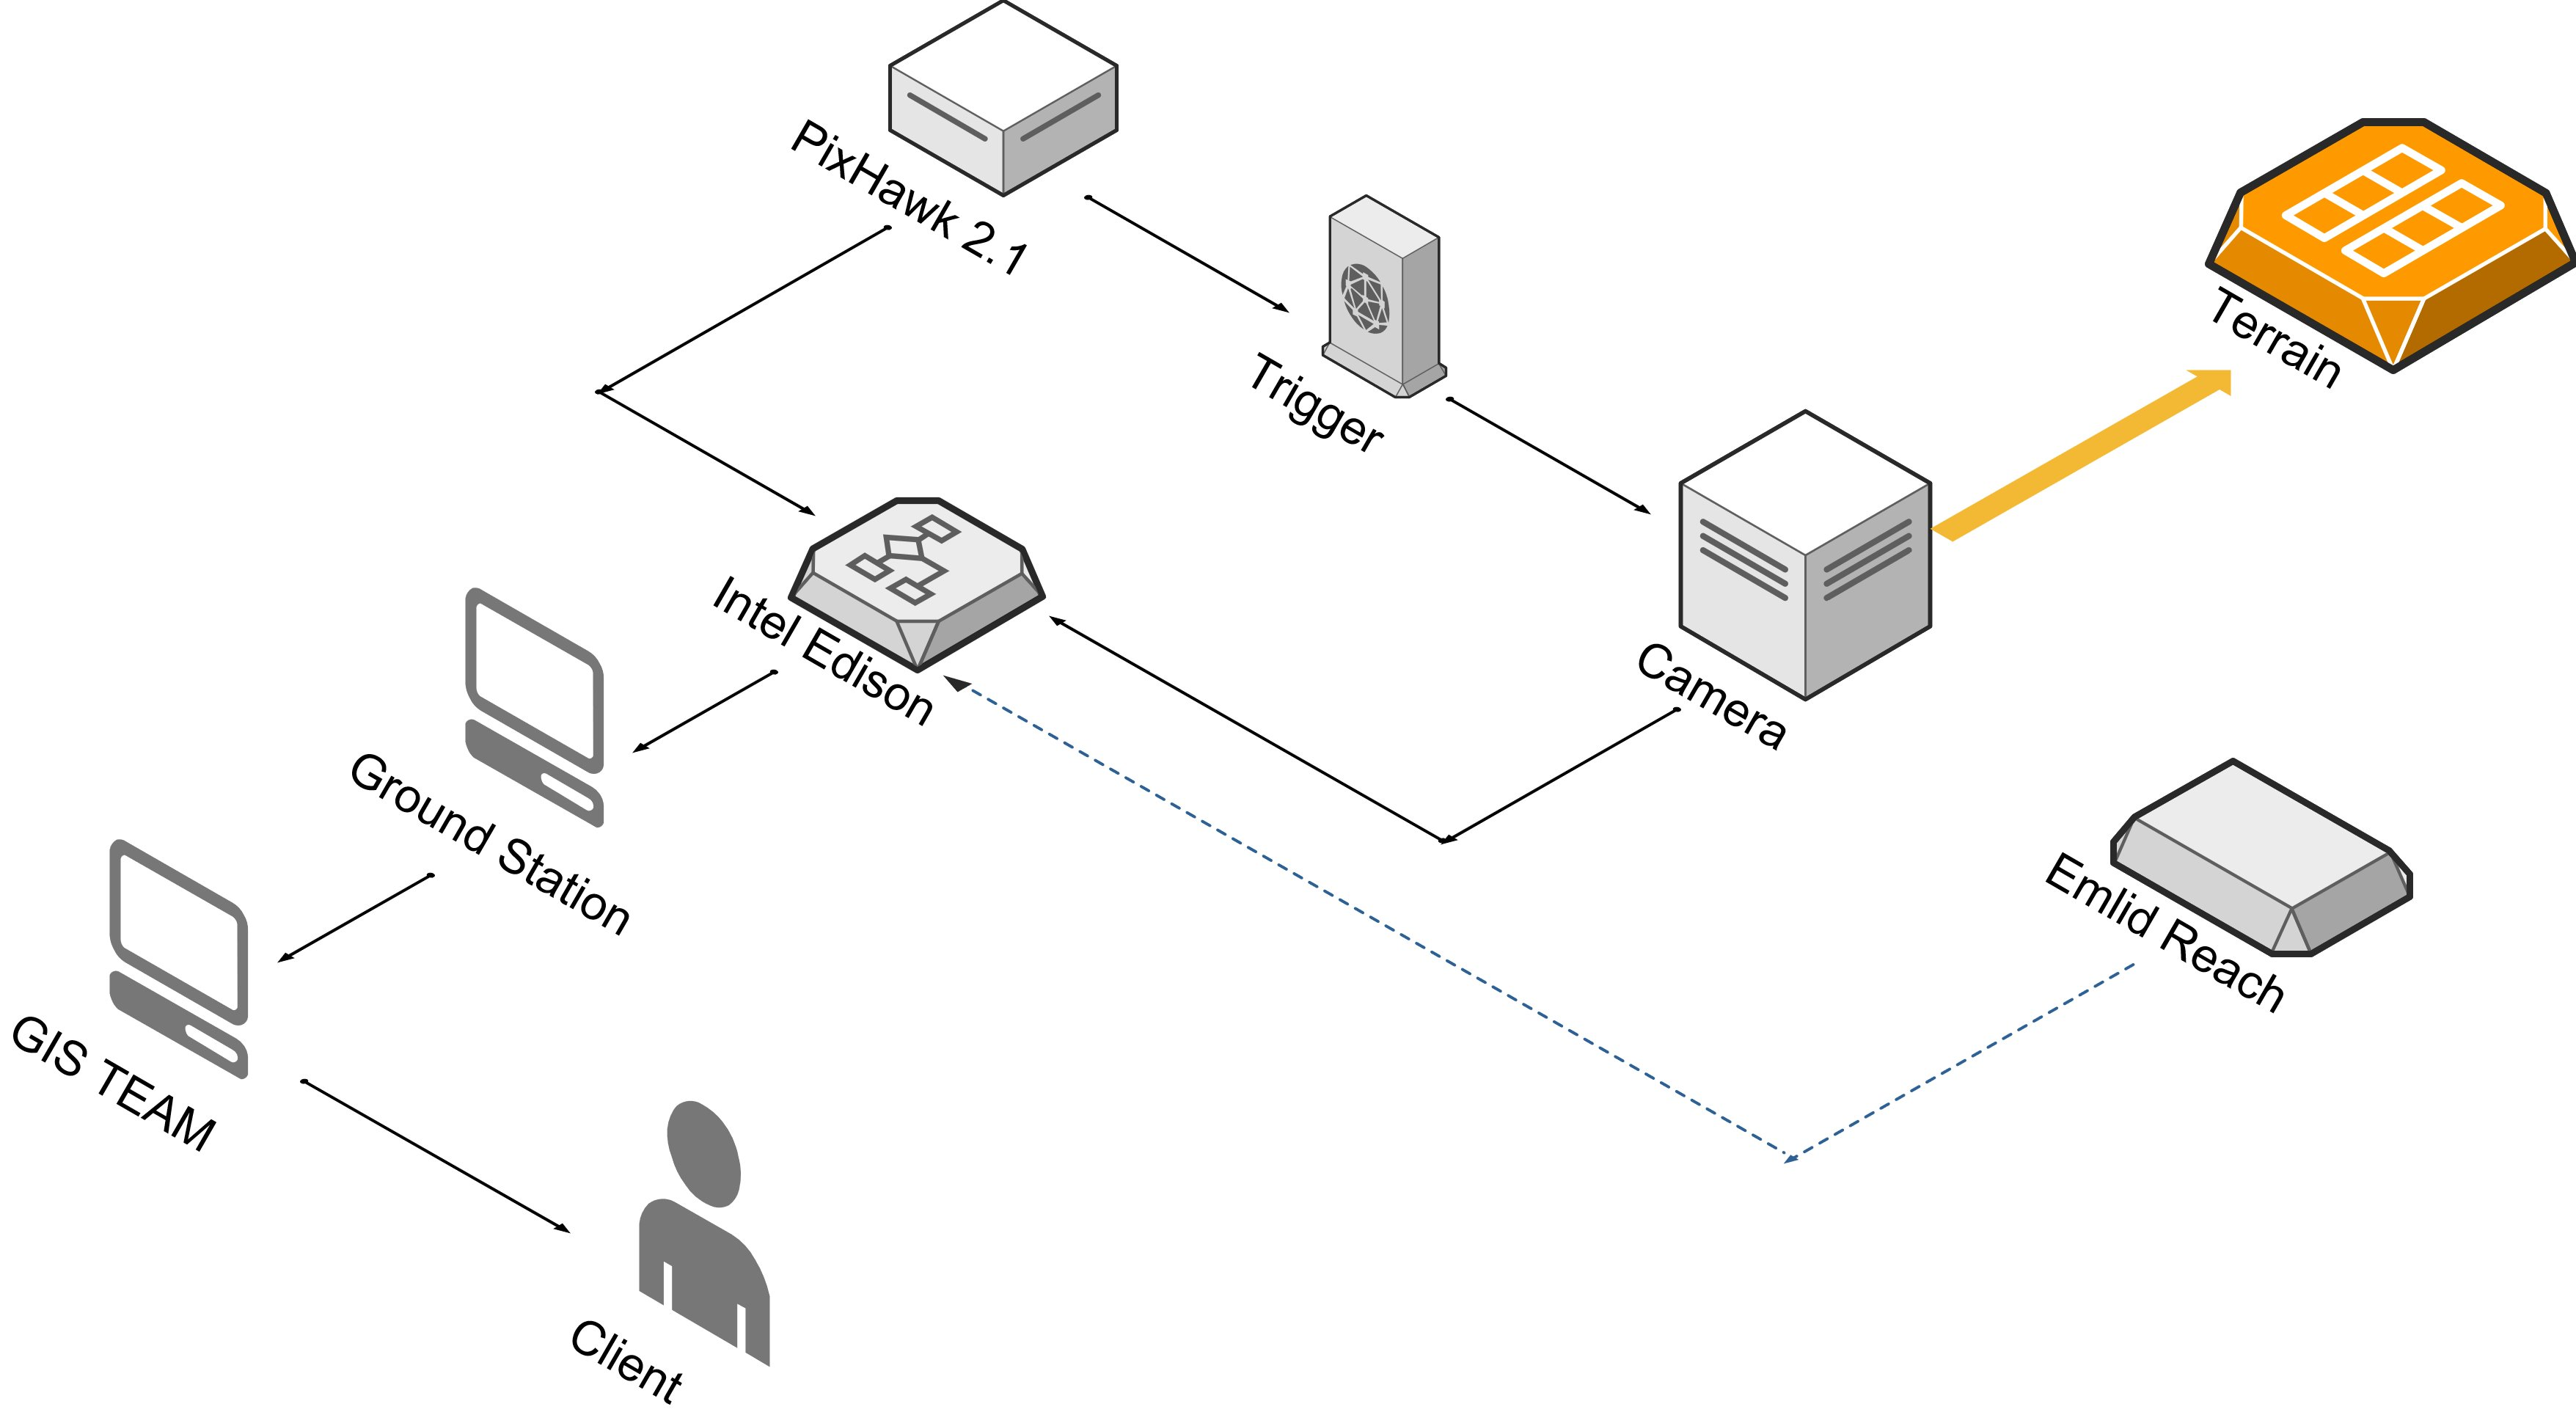
\includegraphics[width=\linewidth]{Alternative_Solution4.jpg}
 \\
 This is similar to the third solution except for the fact that the transfer between the only Intel Edison the ground station communicates with is w\emph{wired}.
\subsection{Advantages}
This has the same advantage as 3 and also there is advantage on the speed of transfer as there will be high speed data transfer.
\subsection{Disadvantages} 
 The only link between ground-station and Intel Edison makes the link of prime importance. DMC might crash if excessive demand falls on this route also the Intel Edison should be successful in fetching the data from PH, camera and the 2 Emlids.
 
\section{Alternate solution b}
 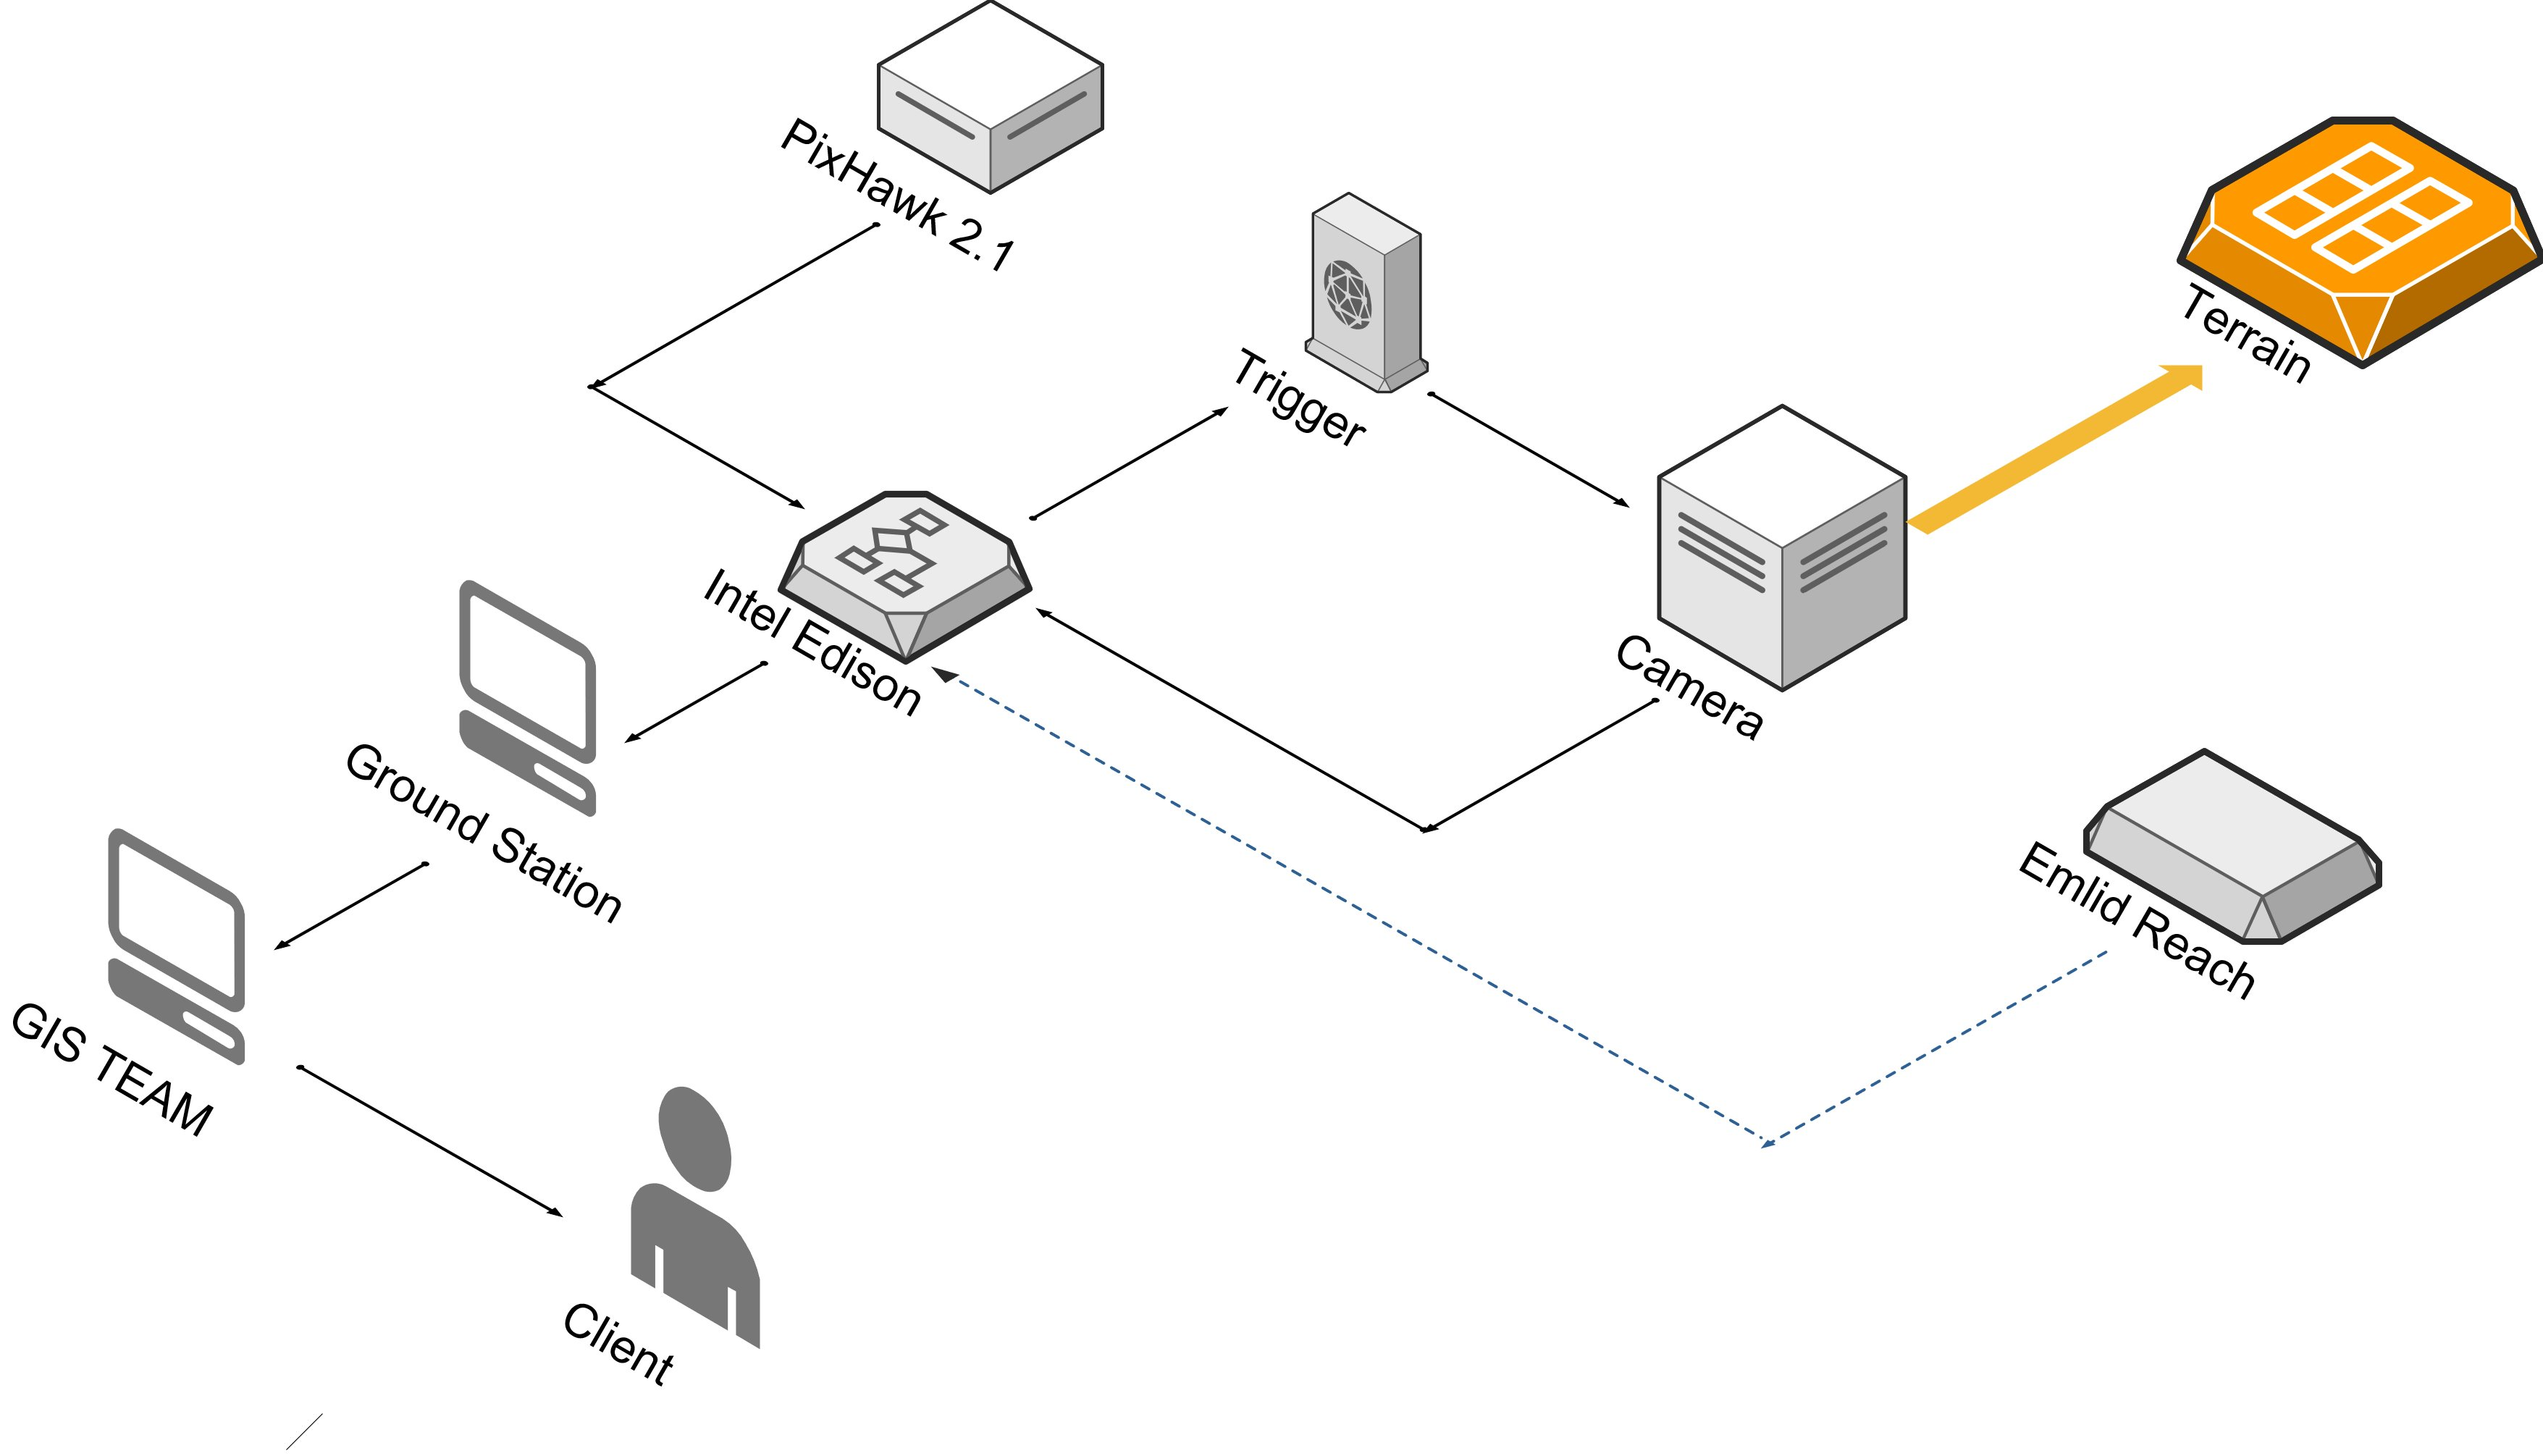
\includegraphics[width=\linewidth]{Alternative_Solution_b.jpg}
This is to say the camera end trigger to be through the micro USB via the Intel Edison. 
\subsection{Advantages}
The hybrid USB needn't be used as devised in Camera solution.
\subsection{Disadvantages} 
There are implementation issues which have not been resolved till now like the switching between USB transfer mode and PC remote mode requires human interaction which is not script replaceable. Also the use of Intel Edison for triger circuit will introduce extra delay in taking snaps which is hard to calculat.
 
 
\section{The chosen solution}
 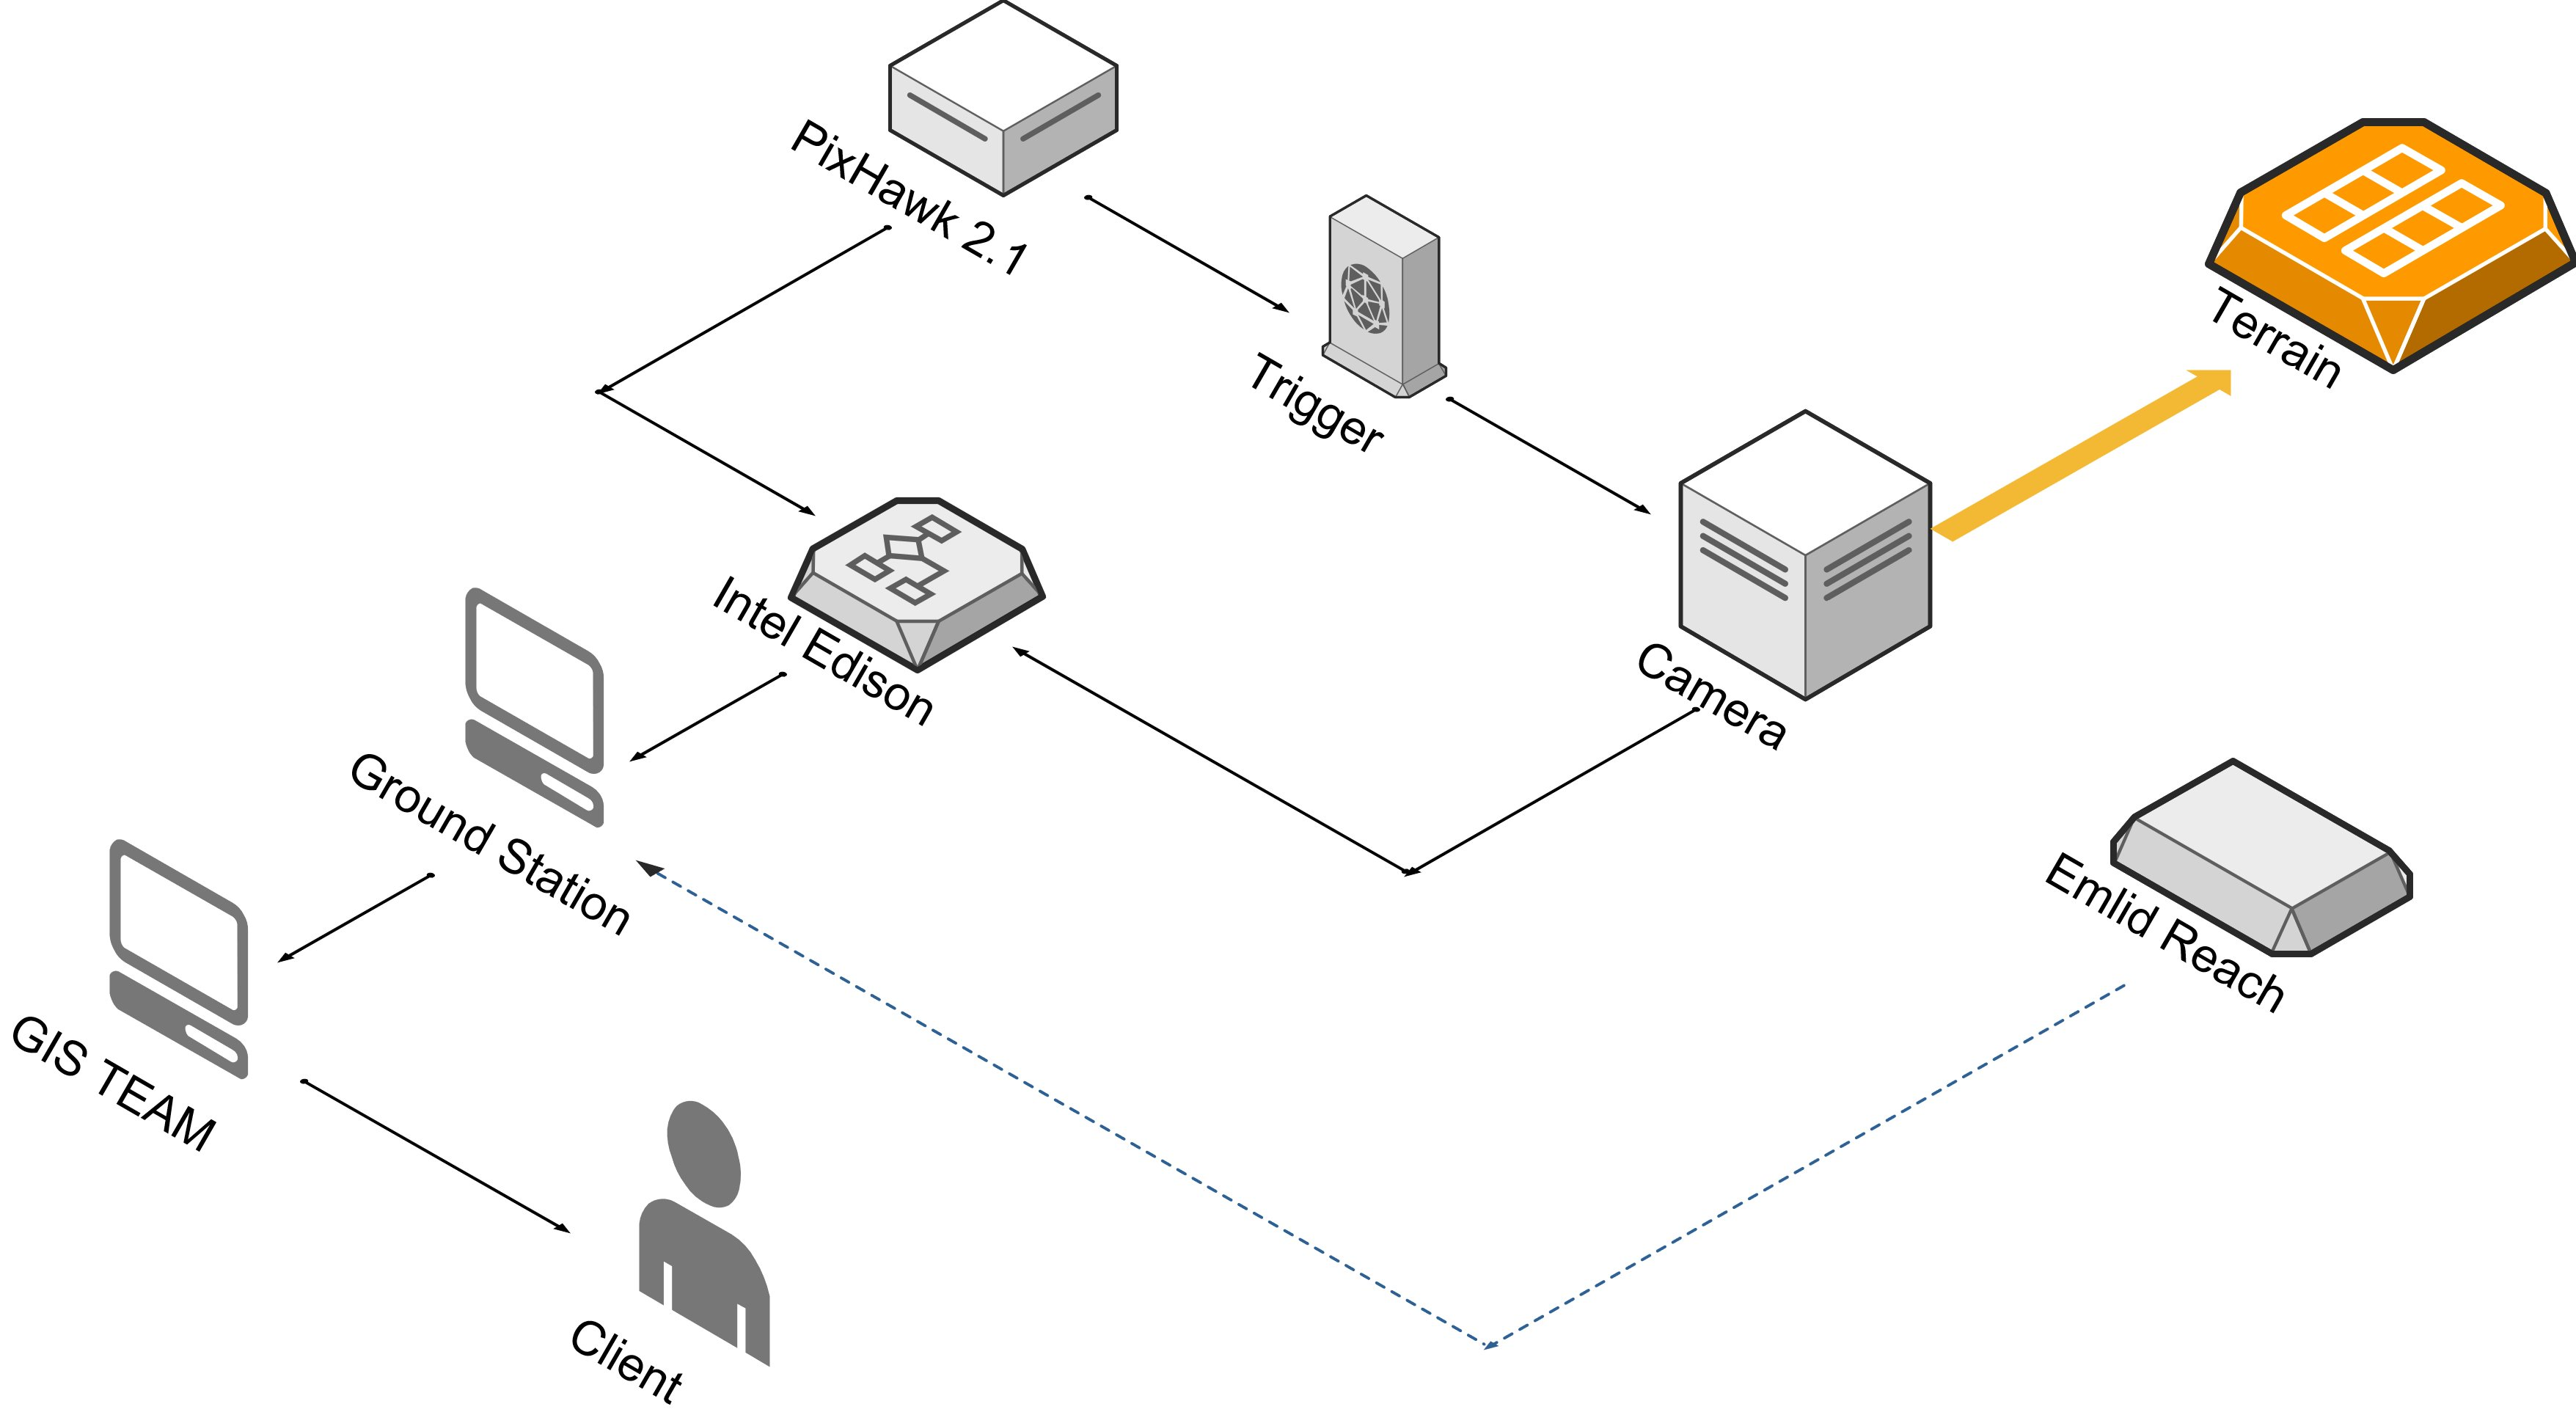
\includegraphics[width=\linewidth]{Alternative_Solution1.jpg} 
After exclusive elimination we are looking forward to use Alternative Solution 1 as shown in the given section.


\chapter{Possibilities you might explore}

%\begin{figure}[!ht]
%\includegraphics[width=\linewidth]{NewFSMfinal.jpg}
%\caption{The FSM after the addition of new Instructions}
%\end{figure}
\begin{itemize}

\item Transfer the log file over WiFi to GroundStation                  -              Assignment 2 \\(http://ardupilot.org/dev/docs/apsync-intro.html)

(Scripts already in E:/Skylark/Work)

On start-up an access point is created with name “ardupilot”. The password is “ardupilot” on TX1 and RPi, “enRouteArduPilot” on the Intel Edison.

The user can connect to this access point and then easily connect to ardupilot running on the flight controller by setting their ground station
 (including Mission Planner) to connect using “UDP”, port 14550.

Dataflash logs are streamed to the companion computer via mavlink and stored on the companion computer’s filesystem (as well as on the pixhawk’s dataflash).
 Dataflash log files can then be quickly downloaded (over wifi) using a script (Windows users may use apsync-download-logs) or you may pull the SD card out
 of the companion computer.

IMPORTANT NOTE: It has been implemented before so not an issue.Just worry about implementing.

\item Get Pictures over WiFi from the Drone:                           -               Assignment 1 \\(http://ardupilot.org/dev/docs/apsync-intro.html)

Data Syncronisation with Web server or Corporate server.
The contents of a configurable list of directories will be automatically uploaded to a configurable web server address.

This should allow the pilot to simply bring the vehicle back in range of a trusted wifi access point, reboot the vehicle and have it 
automatically connect and upload all datafiles including logs, pictures, videos.

IMPORTANT NOTE: The APSync project is still in beta. This Data Syncronisation portion is not implemented (yet). We need to configure data from Camera SD to Edison.



\item Do a lot of processing online using OPEN CV.                     -               Bonus
\\(http://www.instructables.com/id/Getting-Started-With-OpenCV-and-Intel-Edison/)

The Edison pinnout is available all over the place, and there is no restriction from adding additional layers of boards underneath if you would like them.

The Edison it there to do things like smart-shots, controlling a QX1 camera, or a go-pro, or for processing external Lidar data from an SF40 to form a map of an indoor location for example.

the Edison can use any of the IO on the Pixhawk if you program it as such, so it has access to the real world.

the access to the world that it offers, are as follows.

connection via builtin level shifting to serial 2 on the Pixhawk 2 for mavlink communications
Wifi / Bluetooth connection for control, telemetry, camera connectivity etc.
USB OTG for connection to external devices, LTE Modem, Webcam, Lidar, M8T (for PPK GPS)
and of course, the mezzanine method of mounting on the Edison means you could add additional I/O if you so desired.

What I have given you here is a starting point, if you see a use for it, great! but if you don't... that's OK, there are many development boards and other compute modules that will interface just as well as the Edison, some even better, like the Joule, and the TX1

If you have a look at the history of Ardupilot, and the hardware, you will see that hardware is built, people test, the then contribute to the Wiki, and make great stuff from the raw ingredients that we provide.

If you wish to get started with the Edison on Pixhawk 2, go to the wiki... there is a guide their for getting an image working on it.
http://ardupilot.org/dev/docs/intel-edison.html50

it really is a blank canvas for you to do with it what you want. run python scripts, or write your own path planning method... lots of opportunity!

Getting images onto the Intel Edison can be done a couple of different way. You can transfer files using a USB stick, SD card or through an ssh transfer software like FileZilla. However one of the best options is 
to take your pictures with the Intel Edison using a webcam. 
To set up a USB webcam you're going to have to enable UVC support. Luckily there is an in depth tutorial : https://software.intel.com/en-us/articles/opencv-300-beta-ipp-tbb-enabled-on-yocto-with-intel-edison/

Follow this to take Images : https://communities.intel.com/thread/87420 or http://www.instructables.com/id/Intel-Edison-Takes-Pictures-From-Motion-Detection/


BOTTOM LINE: Connect the webcam via the OTG for Edison and get files and run a script to forward it to the Ground Station over WiFi.


\item Basically we can get the PixHawk data, Camera data run combined operations.
\item Additional sensors can be used and data can be fused for better accuracy.
\item Object recognition algorithms to set realistic GCPs
\item RFID tracking
\item Disaster relief supply
\item Create temporary connectivity using drone as a base station
\item Wildlife monitoring
\item A webpage to advertise our services: https://www.dronesden.com/dronehire/
\item Security: Faster response time to 100 dials.
\item Wildlife research
\item Atmospheric research: People are working on studying the ozone layer
\item Chase tornadoes – The Tempest is a UAV that can get reasonably close to a tornado. It is equipped with air pressure, moisture, temperature, and wind speed sensors. The Tempest was able to fly for 44 minutes in a supercell thunderstorm last year, transmitting priceless information to researchers on the ground. 
\item Missile tracers: Suppose a HVT is to be hit and we cannot risk a false lock on as in  some missiles are heat seeking and can be evaded if some other hotter source is nearby(popping flare). However drones equipped with Image Processing techniques can get a true lock on.
\item Rescue operation: A drone equipped with a kinect can be risked to survey a dangerous zone and map the environment in 3 dimensions this will probably give our soldiers an upperhand in a clean swipe/hostage rescue situation. Example: Plan better surgical strikes in Kashmir.
\item Gun/Fire-arm detection: With the power of parallel computing drones can be used to track down infiltrators/explosives. This way counter insurgency operations in J and K area can be handled more efficiently.
\item Drone Sniping: A relatively new area but with excellent Gyroscopes and Control Systems we can probably snipe HVTs with much ease.
\item Fault detection and correction: Lets say a very large structure is manufactured and some small defects are there in weilds with proper sensors and techniques we can rejoin the misaligned joints etc.
\item Facilitate use of simple sensors: Instead of using very expensive sensors we can use raw sensors and use the processing space to detect the thing required. This will allow us to detect and modify algorithms according to our needs. This will emphasize on \emph{reusability}.
\item Good power techniques like use of other fuels than LiPo can revolutionarize the industry as one of the few major concerns are very less flight time.



\end{itemize}

\chapter{Conclusion}
At present we have documented all that has been done and explored in this report and look forward eagerly to use the Intel Edison to make the solutions work and finish my assignment. 



\footnote{Bibliography: discuss.ardupilot.org, Nihal and Nekhelesh's expertise, The team's support }


\end{document}